% Seminarul 14: Active cripto
% Statistica piețelor financiare -- Program de licență, Academia de Studii Economice din București
% GENERAT de latex/build_seminar14.py -- modificați generatorul, nu acest fișier.
% Implicit versiunea pentru studenți; versiunea profesorului este wrapper-ul *_solutions.tex.
\makeatletter\@ifundefined{ifsolutions}{\expandafter\newif\csname ifsolutions\endcsname}{}\makeatother

\newcommand{\coursename}{Statistica piețelor financiare}
\def\sfmlang{ro}
% Preambul comun SFM -- Statistica piețelor financiare / Statistics of Financial Markets (Beamer, 16:9)
% Același design ca MFM. Înainte de % Preambul comun SFM -- Statistica piețelor financiare / Statistics of Financial Markets (Beamer, 16:9)
% Același design ca MFM. Înainte de % Preambul comun SFM -- Statistica piețelor financiare / Statistics of Financial Markets (Beamer, 16:9)
% Același design ca MFM. Înainte de \input{../../latex/preamble} se definește
%   \newcommand{\coursename}{Statistics of Financial Markets}      (EN)
%   \newcommand{\coursename}{Statistica piețelor financiare}       (RO)  și  \def\sfmlang{ro}
% Fișierele .tex se află în EN/Courses, EN/Seminars, RO/Cursuri, RO/Seminarii (două niveluri sub rădăcină).
% Deck-urile sînt generate de latex/build_chapterN.py / build_seminarN.py (vezi latex/sfm_build.py).

\documentclass[9pt, aspectratio=169, t]{beamer}
\providecommand{\coursename}{Statistics of Financial Markets}

% Ensure content fits on slides
\setbeamersize{text margin left=8mm, text margin right=8mm}

%=============================================================================
% THEME AND STYLE CONFIGURATION
%=============================================================================
\usetheme{default}
% Using default theme for clean header/footer control

% Color Palette (matching Redispatch PDF)
\definecolor{MainBlue}{RGB}{26, 58, 110}
\definecolor{AccentBlue}{RGB}{26, 58, 110}
\definecolor{IDAred}{RGB}{205, 0, 0}
\definecolor{DarkGray}{RGB}{51, 51, 51}
\definecolor{MediumGray}{RGB}{128, 128, 128}
\definecolor{LightGray}{RGB}{248, 248, 248}
\definecolor{VeryLightGray}{RGB}{235, 235, 235}
\definecolor{KeynoteGray}{RGB}{218, 218, 218}
\definecolor{SectionGray}{RGB}{120, 120, 120}
\definecolor{FooterGray}{RGB}{100, 100, 100}
\definecolor{Crimson}{RGB}{220, 53, 69}
\definecolor{Forest}{RGB}{46, 125, 50}
\definecolor{Amber}{RGB}{181, 133, 63}
\definecolor{Orange}{RGB}{230, 126, 34}
\definecolor{Purple}{RGB}{142, 68, 173}

% Gradient background (exact Keynote 315° gradient: white to RGB 218,218,218)
\setbeamertemplate{background}{%
    \begin{tikzpicture}[remember picture, overlay]
        \shade[shading=axis, shading angle=315,
        top color=white, bottom color=KeynoteGray]
        (current page.south west) rectangle (current page.north east);
    \end{tikzpicture}%
}
% Fallback solid color for compatibility
\setbeamercolor{background canvas}{bg=}

\setbeamercolor{palette primary}{bg=MainBlue, fg=white}
\setbeamercolor{palette secondary}{bg=MainBlue!85, fg=white}
\setbeamercolor{palette tertiary}{bg=MainBlue!70, fg=white}
\setbeamercolor{structure}{fg=MainBlue}
\setbeamercolor{title}{fg=IDAred}
\setbeamercolor{frametitle}{fg=IDAred, bg=}
\setbeamercolor{block title}{bg=MainBlue, fg=white}
\setbeamercolor{block body}{bg=VeryLightGray, fg=DarkGray}
\setbeamercolor{block title alerted}{bg=Crimson, fg=white}
\setbeamercolor{block body alerted}{bg=Crimson!8, fg=DarkGray}
\setbeamercolor{block title example}{bg=Forest, fg=white}
\setbeamercolor{block body example}{bg=Forest!8, fg=DarkGray}
\setbeamercolor{item}{fg=MainBlue}

% Footer colors (override Madrid theme blue)
\setbeamercolor{author in head/foot}{fg=FooterGray, bg=}
\setbeamercolor{title in head/foot}{fg=FooterGray, bg=}
\setbeamercolor{date in head/foot}{fg=FooterGray, bg=}
\setbeamercolor{section in head/foot}{fg=FooterGray, bg=}
\setbeamercolor{subsection in head/foot}{fg=FooterGray, bg=}

% Bullet styles (apply everywhere including blocks)
\setbeamertemplate{itemize item}{\color{MainBlue}$\boxdot$}
\setbeamertemplate{itemize subitem}{\color{MainBlue}$\blacktriangleright$}
\setbeamertemplate{itemize subsubitem}{\color{MainBlue}\tiny$\bullet$}
\setbeamertemplate{itemize/enumerate body begin}{\normalsize}
\setbeamertemplate{itemize/enumerate subbody begin}{\normalsize}

% Item spacing - compact style
\setlength{\leftmargini}{10pt}       % Level 1: minimal indent
\setlength{\leftmarginii}{10pt}      % Level 2: minimal additional indent
% Compact list spacing (zero extra space before/after lists in blocks)
\makeatletter
\def\@listi{\leftmargin\leftmargini \topsep 0pt \parsep 0pt \itemsep 0pt}
\def\@listii{\leftmargin\leftmarginii \topsep 0pt \parsep 0pt \itemsep 0pt}
\makeatother

\setbeamertemplate{navigation symbols}{}

%=============================================================================
% CUSTOM HEADLINE
%=============================================================================
\setbeamertemplate{headline}{%
    \vskip10pt%
    \hbox to \paperwidth{%
        \hskip0.5cm%
        {\small\color{FooterGray}\renewcommand{\hyperlink}[2]{##2}\insertsectionhead}%
        \hfill%
        \textcolor{FooterGray}{\small\insertframenumber}%
        \hskip0.5cm%
    }%
    \vskip4pt%
    {\color{FooterGray}\hrule height 0.4pt}%
}

%=============================================================================
% CUSTOM FOOTER
%=============================================================================
\usepackage{fontawesome5}

\setbeamertemplate{footline}{%
    {\color{FooterGray}\hrule height 0.4pt}%
    \vskip4pt%
    \hbox to \paperwidth{%
        \hskip0.5cm%
        \textcolor{FooterGray}{\small\coursename}%
        \hfill%
        \raisebox{-0.1em}{%
            \begin{tikzpicture}[x=0.08em, y=0.08em, line width=0.4pt]
                \draw[FooterGray] (0,3) -- (1,4) -- (2,3.5) -- (3,5) -- (4,4) -- (5,6) -- (6,5.5) -- (7,4) -- (8,5) -- (9,7) -- (10,6) -- (11,5) -- (12,6.5) -- (13,8) -- (14,7) -- (15,6) -- (16,7.5) -- (17,9) -- (18,8) -- (19,7) -- (20,8.5) -- (21,10) -- (22,9) -- (23,8) -- (24,9.5);
            \end{tikzpicture}%
        }%
        \hskip0.5cm%
    }%
    \vskip6pt%
}

%=============================================================================
% PACKAGES
%=============================================================================
\usepackage[utf8]{inputenc}
\DeclareUnicodeCharacter{03B1}{\ensuremath{\alpha}}
\usepackage[T1]{fontenc}
\usepackage{amsmath, amssymb, amsthm}
\usepackage{mathtools}
\usepackage{bm}
\usepackage{tikz}
\usetikzlibrary{arrows.meta, positioning, shapes, calc, decorations.pathreplacing, shadings}
\usepackage{booktabs}
\usepackage{multirow}
\usepackage{array}
\usepackage{graphicx}
\usepackage{hyperref}
\usepackage{colortbl}
\usepackage{listings}
\lstset{language=Python, basicstyle=\ttfamily\scriptsize, keywordstyle=\color{MainBlue}\bfseries,
  commentstyle=\color{Forest}, stringstyle=\color{Crimson}, breaklines=true,
  frame=none, backgroundcolor=\color{VeryLightGray}, xleftmargin=2mm}
\hypersetup{colorlinks=true, linkcolor=MainBlue, urlcolor=MainBlue}
\graphicspath{{../../logos/}{../../charts/}{../../photos/}}
\usepackage{xcolor}
\hfuzz=2pt  % Suppress tiny overfull warnings (<2pt)
\vfuzz=2pt  % Suppress tiny vertical overfull warnings (<2pt)

%=============================================================================
% QUANTLET COMMANDS
%   \quantlet{<displayed name>}{<url>}       (generic, compatible with the older SFM decks)
%   \sfmquantlet{Ch_05}{SFM_ch5_garch}       -> https://github.com/danpele/SFM/tree/main/Quantlets/Ch_05/SFM_ch5_garch
%   \qlurl{<folder>} is defined per chapter by the generator (Quantlets/Ch_NN/<folder>)
%=============================================================================
\newcommand{\sfmrepo}{https://github.com/danpele/SFM}
\newcommand{\sfmqlbase}{https://github.com/danpele/SFM/tree/main/Quantlets}
\newcommand{\quantlet}[2]{%
    \hfill\href{#2}{%
        \raisebox{-0.15em}{
\includegraphics[height=0.7em]{ql_logo.png}}%
        \textcolor{MainBlue}{\tiny\ #1}%
    }%
}
\newcommand{\sfmquantlet}[2]{\quantlet{\detokenize{#2}}{\sfmqlbase/#1/#2}}

%=============================================================================
% NOTEBOOKS (Google Colab)
%   \colaburl{notebooks/EN/chapter5_seminar_notebook.ipynb} -> the Colab link of a file in the SFM repo
%   \nb: the chapter notebook (each seminar deck redefines it with \renewcommand)
%=============================================================================
\newcommand{\colaburl}[1]{https://colab.research.google.com/github/danpele/SFM/blob/main/#1}
\newcommand{\nb}{https://colab.research.google.com/github/danpele/SFM/tree/main/notebooks/EN}
\newcommand{\nbname}{notebooks/EN}

%=============================================================================
% SLIDE HELPERS (used by the generators; the same as in MFM)
%=============================================================================
% local font size for list bodies (the preamble forces \normalsize)
\newcommand{\itemsize}[1]{\setbeamertemplate{itemize/enumerate body begin}{#1}\setbeamertemplate{itemize/enumerate subbody begin}{#1}}
\newcommand{\intitle}[1]{{\hypersetup{urlcolor=white}#1}}   % white links inside coloured title bars
\newcommand{\imgcap}[1]{{\scriptsize #1}\\[0.5mm]}          % caption under a photo
\newcommand{\imgcredit}[2]{{\tiny\color{FooterGray}\href{#1}{#2}}}   % image credit: source URL, author/licence
\newcommand{\aiprompt}[1]{{\ttfamily\color{MainBlue}#1}}     % a prompt to an AI assistant

%=============================================================================
% SEMINARS: student version by default; the instructor wrapper *_solutions.tex sets \solutionstrue
%=============================================================================
\makeatletter\@ifundefined{ifsolutions}{\expandafter\newif\csname ifsolutions\endcsname}{}\makeatother
\newcommand{\solonly}[1]{\ifsolutions #1\fi}
\newcommand{\propsub}{\ifsolutions\else\framesubtitle{\ifdefined\sfmlang Rezolvarea se discută la seminar\else Solution discussed in class\fi}\fi}

%=============================================================================
% APPENDIX AND CHAPTER LINKS (latex/appendix_links.py writes the calls; it also re-declares these
% macros before \begin{document}, so the decks compile with or without this preamble block)
%=============================================================================
\providecommand{\sfmapplink}[3]{\hypertarget{#2}{}\hyperlink{#1}{\beamergotobutton{#3}}}
\providecommand{\sfmappback}[2]{\begin{tikzpicture}[remember picture,overlay]\node[anchor=south east] at ([xshift=-3mm,yshift=7mm]current page.south east){\hyperlink{#1}{\beamerreturnbutton{#2}}};\end{tikzpicture}}
\providecommand{\sfmchlink}[2]{\href{#1}{#2}}
\providecommand{\sfmchlinkt}[2]{\href{#1}{\usebeamercolor[fg]{frametitle}#2}}

%=============================================================================
% QUANTINAR COMMAND: link către un curs Quantinar (subiecte avansate)
%=============================================================================
\newcommand{\quantinar}[2]{%
    \href{#2}{%
        \raisebox{-0.15em}{
\includegraphics[height=0.8em]{qr_logo.png}}%
        \textcolor{MainBlue}{\scriptsize\ #1}%
    }%
}

%=============================================================================
% CUSTOM TITLE PAGE
%=============================================================================
\defbeamertemplate*{title page}{hybrid}[1][]
{
    \vspace{0.2cm}
    % Logos row - top header (with clickable links)
    \begin{center}
        \href{https://www.ase.ro}{
\includegraphics[height=1.0cm]{ase_logo.png}}\hspace{0.3cm}%
        \href{https://theida.net}{
\includegraphics[height=1.0cm]{ida_logo.png}}\hspace{0.3cm}%
        \href{https://blockchain-research-center.com}{
\includegraphics[height=1.0cm]{brc_logo.png}}\hspace{0.3cm}%
        \href{https://www.ai4efin.ase.ro}{
\includegraphics[height=1.0cm]{ai4efin_logo.png}}\hspace{0.3cm}%
        \href{https://ipe.ro/new}{
\includegraphics[height=1.0cm]{acad_logo.png}}\hspace{0.3cm}%
        \href{https://www.digital-finance-msca.com}{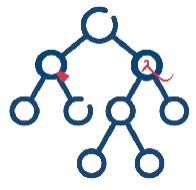
\includegraphics[height=1.0cm]{msca_logo.png}}%
    \end{center}

    \vspace{0.6cm}

    % Main title with Q logos on sides (with clickable links)
    \begin{center}
        \begin{minipage}{0.1\textwidth}
            \centering
            \href{https://quantlet.com}{
\includegraphics[height=1.1cm]{ql_logo.png}}
        \end{minipage}%
        \begin{minipage}{0.78\textwidth}
            \centering
            {\LARGE\bfseries\usebeamercolor[fg]{title}\inserttitle}

            \vspace{0.3cm}

            {\usebeamerfont{subtitle}\usebeamercolor[fg]{title}\insertsubtitle}
        \end{minipage}%
        \begin{minipage}{0.1\textwidth}
            \centering
            \href{https://quantinar.com}{
\includegraphics[height=1.1cm]{qr_logo.png}}
        \end{minipage}
    \end{center}

    \vspace{0.6cm}

    % Authors (left aligned)
    \hspace{0.5cm}{\usebeamerfont{author}\insertauthor}

    \vspace{0.3cm}

    % Institute/Affiliations (left aligned)
    \hspace{0.5cm}\begin{minipage}[t]{0.9\textwidth}
        \raggedright\small\insertinstitute
    \end{minipage}
}

%=============================================================================
% THEOREM ENVIRONMENTS
%=============================================================================
\theoremstyle{definition}
\setbeamertemplate{theorems}[numbered]
\ifdefined\sfmlang
\newtheorem{defn}{Definiție}
\newtheorem{thm}{Teoremă}
\newtheorem{prop}{Propoziție}
\newtheorem{rmk}{Observație}
\else
\newtheorem{defn}{Definition}
\newtheorem{thm}{Theorem}
\newtheorem{prop}{Proposition}
\newtheorem{rmk}{Remark}
\fi

%=============================================================================
% CENTRED MINIPAGE (no extra vertical space)
%=============================================================================
\newenvironment{cminipage}[1]{%
    \par\noindent\hfill\begin{minipage}{#1}\ignorespaces
}{%
    \end{minipage}\hfill\null\par
}

%=============================================================================
% CUSTOM COMMANDS
%=============================================================================
\newcommand{\E}{\mathbb{E}}
\newcommand{\Var}{\text{Var}}
\newcommand{\Cov}{\text{Cov}}
\newcommand{\Corr}{\text{Corr}}
\newcommand{\R}{\mathbb{R}}
\newcommand{\N}{\mathbb{N}}
\newcommand{\Z}{\mathbb{Z}}
\newcommand{\B}{\mathbf{B}}
\newcommand{\imark}{\textcolor{MainBlue}{\textbullet}}
\newcommand{\RMSE}{\text{RMSE}}
\newcommand{\MAE}{\text{MAE}}
\newcommand{\MAPE}{\text{MAPE}}

 se definește
%   \newcommand{\coursename}{Statistics of Financial Markets}      (EN)
%   \newcommand{\coursename}{Statistica piețelor financiare}       (RO)  și  \def\sfmlang{ro}
% Fișierele .tex se află în EN/Courses, EN/Seminars, RO/Cursuri, RO/Seminarii (două niveluri sub rădăcină).
% Deck-urile sînt generate de latex/build_chapterN.py / build_seminarN.py (vezi latex/sfm_build.py).

\documentclass[9pt, aspectratio=169, t]{beamer}
\providecommand{\coursename}{Statistics of Financial Markets}

% Ensure content fits on slides
\setbeamersize{text margin left=8mm, text margin right=8mm}

%=============================================================================
% THEME AND STYLE CONFIGURATION
%=============================================================================
\usetheme{default}
% Using default theme for clean header/footer control

% Color Palette (matching Redispatch PDF)
\definecolor{MainBlue}{RGB}{26, 58, 110}
\definecolor{AccentBlue}{RGB}{26, 58, 110}
\definecolor{IDAred}{RGB}{205, 0, 0}
\definecolor{DarkGray}{RGB}{51, 51, 51}
\definecolor{MediumGray}{RGB}{128, 128, 128}
\definecolor{LightGray}{RGB}{248, 248, 248}
\definecolor{VeryLightGray}{RGB}{235, 235, 235}
\definecolor{KeynoteGray}{RGB}{218, 218, 218}
\definecolor{SectionGray}{RGB}{120, 120, 120}
\definecolor{FooterGray}{RGB}{100, 100, 100}
\definecolor{Crimson}{RGB}{220, 53, 69}
\definecolor{Forest}{RGB}{46, 125, 50}
\definecolor{Amber}{RGB}{181, 133, 63}
\definecolor{Orange}{RGB}{230, 126, 34}
\definecolor{Purple}{RGB}{142, 68, 173}

% Gradient background (exact Keynote 315° gradient: white to RGB 218,218,218)
\setbeamertemplate{background}{%
    \begin{tikzpicture}[remember picture, overlay]
        \shade[shading=axis, shading angle=315,
        top color=white, bottom color=KeynoteGray]
        (current page.south west) rectangle (current page.north east);
    \end{tikzpicture}%
}
% Fallback solid color for compatibility
\setbeamercolor{background canvas}{bg=}

\setbeamercolor{palette primary}{bg=MainBlue, fg=white}
\setbeamercolor{palette secondary}{bg=MainBlue!85, fg=white}
\setbeamercolor{palette tertiary}{bg=MainBlue!70, fg=white}
\setbeamercolor{structure}{fg=MainBlue}
\setbeamercolor{title}{fg=IDAred}
\setbeamercolor{frametitle}{fg=IDAred, bg=}
\setbeamercolor{block title}{bg=MainBlue, fg=white}
\setbeamercolor{block body}{bg=VeryLightGray, fg=DarkGray}
\setbeamercolor{block title alerted}{bg=Crimson, fg=white}
\setbeamercolor{block body alerted}{bg=Crimson!8, fg=DarkGray}
\setbeamercolor{block title example}{bg=Forest, fg=white}
\setbeamercolor{block body example}{bg=Forest!8, fg=DarkGray}
\setbeamercolor{item}{fg=MainBlue}

% Footer colors (override Madrid theme blue)
\setbeamercolor{author in head/foot}{fg=FooterGray, bg=}
\setbeamercolor{title in head/foot}{fg=FooterGray, bg=}
\setbeamercolor{date in head/foot}{fg=FooterGray, bg=}
\setbeamercolor{section in head/foot}{fg=FooterGray, bg=}
\setbeamercolor{subsection in head/foot}{fg=FooterGray, bg=}

% Bullet styles (apply everywhere including blocks)
\setbeamertemplate{itemize item}{\color{MainBlue}$\boxdot$}
\setbeamertemplate{itemize subitem}{\color{MainBlue}$\blacktriangleright$}
\setbeamertemplate{itemize subsubitem}{\color{MainBlue}\tiny$\bullet$}
\setbeamertemplate{itemize/enumerate body begin}{\normalsize}
\setbeamertemplate{itemize/enumerate subbody begin}{\normalsize}

% Item spacing - compact style
\setlength{\leftmargini}{10pt}       % Level 1: minimal indent
\setlength{\leftmarginii}{10pt}      % Level 2: minimal additional indent
% Compact list spacing (zero extra space before/after lists in blocks)
\makeatletter
\def\@listi{\leftmargin\leftmargini \topsep 0pt \parsep 0pt \itemsep 0pt}
\def\@listii{\leftmargin\leftmarginii \topsep 0pt \parsep 0pt \itemsep 0pt}
\makeatother

\setbeamertemplate{navigation symbols}{}

%=============================================================================
% CUSTOM HEADLINE
%=============================================================================
\setbeamertemplate{headline}{%
    \vskip10pt%
    \hbox to \paperwidth{%
        \hskip0.5cm%
        {\small\color{FooterGray}\renewcommand{\hyperlink}[2]{##2}\insertsectionhead}%
        \hfill%
        \textcolor{FooterGray}{\small\insertframenumber}%
        \hskip0.5cm%
    }%
    \vskip4pt%
    {\color{FooterGray}\hrule height 0.4pt}%
}

%=============================================================================
% CUSTOM FOOTER
%=============================================================================
\usepackage{fontawesome5}

\setbeamertemplate{footline}{%
    {\color{FooterGray}\hrule height 0.4pt}%
    \vskip4pt%
    \hbox to \paperwidth{%
        \hskip0.5cm%
        \textcolor{FooterGray}{\small\coursename}%
        \hfill%
        \raisebox{-0.1em}{%
            \begin{tikzpicture}[x=0.08em, y=0.08em, line width=0.4pt]
                \draw[FooterGray] (0,3) -- (1,4) -- (2,3.5) -- (3,5) -- (4,4) -- (5,6) -- (6,5.5) -- (7,4) -- (8,5) -- (9,7) -- (10,6) -- (11,5) -- (12,6.5) -- (13,8) -- (14,7) -- (15,6) -- (16,7.5) -- (17,9) -- (18,8) -- (19,7) -- (20,8.5) -- (21,10) -- (22,9) -- (23,8) -- (24,9.5);
            \end{tikzpicture}%
        }%
        \hskip0.5cm%
    }%
    \vskip6pt%
}

%=============================================================================
% PACKAGES
%=============================================================================
\usepackage[utf8]{inputenc}
\DeclareUnicodeCharacter{03B1}{\ensuremath{\alpha}}
\usepackage[T1]{fontenc}
\usepackage{amsmath, amssymb, amsthm}
\usepackage{mathtools}
\usepackage{bm}
\usepackage{tikz}
\usetikzlibrary{arrows.meta, positioning, shapes, calc, decorations.pathreplacing, shadings}
\usepackage{booktabs}
\usepackage{multirow}
\usepackage{array}
\usepackage{graphicx}
\usepackage{hyperref}
\usepackage{colortbl}
\usepackage{listings}
\lstset{language=Python, basicstyle=\ttfamily\scriptsize, keywordstyle=\color{MainBlue}\bfseries,
  commentstyle=\color{Forest}, stringstyle=\color{Crimson}, breaklines=true,
  frame=none, backgroundcolor=\color{VeryLightGray}, xleftmargin=2mm}
\hypersetup{colorlinks=true, linkcolor=MainBlue, urlcolor=MainBlue}
\graphicspath{{../../logos/}{../../charts/}{../../photos/}}
\usepackage{xcolor}
\hfuzz=2pt  % Suppress tiny overfull warnings (<2pt)
\vfuzz=2pt  % Suppress tiny vertical overfull warnings (<2pt)

%=============================================================================
% QUANTLET COMMANDS
%   \quantlet{<displayed name>}{<url>}       (generic, compatible with the older SFM decks)
%   \sfmquantlet{Ch_05}{SFM_ch5_garch}       -> https://github.com/danpele/SFM/tree/main/Quantlets/Ch_05/SFM_ch5_garch
%   \qlurl{<folder>} is defined per chapter by the generator (Quantlets/Ch_NN/<folder>)
%=============================================================================
\newcommand{\sfmrepo}{https://github.com/danpele/SFM}
\newcommand{\sfmqlbase}{https://github.com/danpele/SFM/tree/main/Quantlets}
\newcommand{\quantlet}[2]{%
    \hfill\href{#2}{%
        \raisebox{-0.15em}{
\includegraphics[height=0.7em]{ql_logo.png}}%
        \textcolor{MainBlue}{\tiny\ #1}%
    }%
}
\newcommand{\sfmquantlet}[2]{\quantlet{\detokenize{#2}}{\sfmqlbase/#1/#2}}

%=============================================================================
% NOTEBOOKS (Google Colab)
%   \colaburl{notebooks/EN/chapter5_seminar_notebook.ipynb} -> the Colab link of a file in the SFM repo
%   \nb: the chapter notebook (each seminar deck redefines it with \renewcommand)
%=============================================================================
\newcommand{\colaburl}[1]{https://colab.research.google.com/github/danpele/SFM/blob/main/#1}
\newcommand{\nb}{https://colab.research.google.com/github/danpele/SFM/tree/main/notebooks/EN}
\newcommand{\nbname}{notebooks/EN}

%=============================================================================
% SLIDE HELPERS (used by the generators; the same as in MFM)
%=============================================================================
% local font size for list bodies (the preamble forces \normalsize)
\newcommand{\itemsize}[1]{\setbeamertemplate{itemize/enumerate body begin}{#1}\setbeamertemplate{itemize/enumerate subbody begin}{#1}}
\newcommand{\intitle}[1]{{\hypersetup{urlcolor=white}#1}}   % white links inside coloured title bars
\newcommand{\imgcap}[1]{{\scriptsize #1}\\[0.5mm]}          % caption under a photo
\newcommand{\imgcredit}[2]{{\tiny\color{FooterGray}\href{#1}{#2}}}   % image credit: source URL, author/licence
\newcommand{\aiprompt}[1]{{\ttfamily\color{MainBlue}#1}}     % a prompt to an AI assistant

%=============================================================================
% SEMINARS: student version by default; the instructor wrapper *_solutions.tex sets \solutionstrue
%=============================================================================
\makeatletter\@ifundefined{ifsolutions}{\expandafter\newif\csname ifsolutions\endcsname}{}\makeatother
\newcommand{\solonly}[1]{\ifsolutions #1\fi}
\newcommand{\propsub}{\ifsolutions\else\framesubtitle{\ifdefined\sfmlang Rezolvarea se discută la seminar\else Solution discussed in class\fi}\fi}

%=============================================================================
% APPENDIX AND CHAPTER LINKS (latex/appendix_links.py writes the calls; it also re-declares these
% macros before \begin{document}, so the decks compile with or without this preamble block)
%=============================================================================
\providecommand{\sfmapplink}[3]{\hypertarget{#2}{}\hyperlink{#1}{\beamergotobutton{#3}}}
\providecommand{\sfmappback}[2]{\begin{tikzpicture}[remember picture,overlay]\node[anchor=south east] at ([xshift=-3mm,yshift=7mm]current page.south east){\hyperlink{#1}{\beamerreturnbutton{#2}}};\end{tikzpicture}}
\providecommand{\sfmchlink}[2]{\href{#1}{#2}}
\providecommand{\sfmchlinkt}[2]{\href{#1}{\usebeamercolor[fg]{frametitle}#2}}

%=============================================================================
% QUANTINAR COMMAND: link către un curs Quantinar (subiecte avansate)
%=============================================================================
\newcommand{\quantinar}[2]{%
    \href{#2}{%
        \raisebox{-0.15em}{
\includegraphics[height=0.8em]{qr_logo.png}}%
        \textcolor{MainBlue}{\scriptsize\ #1}%
    }%
}

%=============================================================================
% CUSTOM TITLE PAGE
%=============================================================================
\defbeamertemplate*{title page}{hybrid}[1][]
{
    \vspace{0.2cm}
    % Logos row - top header (with clickable links)
    \begin{center}
        \href{https://www.ase.ro}{
\includegraphics[height=1.0cm]{ase_logo.png}}\hspace{0.3cm}%
        \href{https://theida.net}{
\includegraphics[height=1.0cm]{ida_logo.png}}\hspace{0.3cm}%
        \href{https://blockchain-research-center.com}{
\includegraphics[height=1.0cm]{brc_logo.png}}\hspace{0.3cm}%
        \href{https://www.ai4efin.ase.ro}{
\includegraphics[height=1.0cm]{ai4efin_logo.png}}\hspace{0.3cm}%
        \href{https://ipe.ro/new}{
\includegraphics[height=1.0cm]{acad_logo.png}}\hspace{0.3cm}%
        \href{https://www.digital-finance-msca.com}{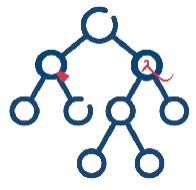
\includegraphics[height=1.0cm]{msca_logo.png}}%
    \end{center}

    \vspace{0.6cm}

    % Main title with Q logos on sides (with clickable links)
    \begin{center}
        \begin{minipage}{0.1\textwidth}
            \centering
            \href{https://quantlet.com}{
\includegraphics[height=1.1cm]{ql_logo.png}}
        \end{minipage}%
        \begin{minipage}{0.78\textwidth}
            \centering
            {\LARGE\bfseries\usebeamercolor[fg]{title}\inserttitle}

            \vspace{0.3cm}

            {\usebeamerfont{subtitle}\usebeamercolor[fg]{title}\insertsubtitle}
        \end{minipage}%
        \begin{minipage}{0.1\textwidth}
            \centering
            \href{https://quantinar.com}{
\includegraphics[height=1.1cm]{qr_logo.png}}
        \end{minipage}
    \end{center}

    \vspace{0.6cm}

    % Authors (left aligned)
    \hspace{0.5cm}{\usebeamerfont{author}\insertauthor}

    \vspace{0.3cm}

    % Institute/Affiliations (left aligned)
    \hspace{0.5cm}\begin{minipage}[t]{0.9\textwidth}
        \raggedright\small\insertinstitute
    \end{minipage}
}

%=============================================================================
% THEOREM ENVIRONMENTS
%=============================================================================
\theoremstyle{definition}
\setbeamertemplate{theorems}[numbered]
\ifdefined\sfmlang
\newtheorem{defn}{Definiție}
\newtheorem{thm}{Teoremă}
\newtheorem{prop}{Propoziție}
\newtheorem{rmk}{Observație}
\else
\newtheorem{defn}{Definition}
\newtheorem{thm}{Theorem}
\newtheorem{prop}{Proposition}
\newtheorem{rmk}{Remark}
\fi

%=============================================================================
% CENTRED MINIPAGE (no extra vertical space)
%=============================================================================
\newenvironment{cminipage}[1]{%
    \par\noindent\hfill\begin{minipage}{#1}\ignorespaces
}{%
    \end{minipage}\hfill\null\par
}

%=============================================================================
% CUSTOM COMMANDS
%=============================================================================
\newcommand{\E}{\mathbb{E}}
\newcommand{\Var}{\text{Var}}
\newcommand{\Cov}{\text{Cov}}
\newcommand{\Corr}{\text{Corr}}
\newcommand{\R}{\mathbb{R}}
\newcommand{\N}{\mathbb{N}}
\newcommand{\Z}{\mathbb{Z}}
\newcommand{\B}{\mathbf{B}}
\newcommand{\imark}{\textcolor{MainBlue}{\textbullet}}
\newcommand{\RMSE}{\text{RMSE}}
\newcommand{\MAE}{\text{MAE}}
\newcommand{\MAPE}{\text{MAPE}}

 se definește
%   \newcommand{\coursename}{Statistics of Financial Markets}      (EN)
%   \newcommand{\coursename}{Statistica piețelor financiare}       (RO)  și  \def\sfmlang{ro}
% Fișierele .tex se află în EN/Courses, EN/Seminars, RO/Cursuri, RO/Seminarii (două niveluri sub rădăcină).
% Deck-urile sînt generate de latex/build_chapterN.py / build_seminarN.py (vezi latex/sfm_build.py).

\documentclass[9pt, aspectratio=169, t]{beamer}
\providecommand{\coursename}{Statistics of Financial Markets}

% Ensure content fits on slides
\setbeamersize{text margin left=8mm, text margin right=8mm}

%=============================================================================
% THEME AND STYLE CONFIGURATION
%=============================================================================
\usetheme{default}
% Using default theme for clean header/footer control

% Color Palette (matching Redispatch PDF)
\definecolor{MainBlue}{RGB}{26, 58, 110}
\definecolor{AccentBlue}{RGB}{26, 58, 110}
\definecolor{IDAred}{RGB}{205, 0, 0}
\definecolor{DarkGray}{RGB}{51, 51, 51}
\definecolor{MediumGray}{RGB}{128, 128, 128}
\definecolor{LightGray}{RGB}{248, 248, 248}
\definecolor{VeryLightGray}{RGB}{235, 235, 235}
\definecolor{KeynoteGray}{RGB}{218, 218, 218}
\definecolor{SectionGray}{RGB}{120, 120, 120}
\definecolor{FooterGray}{RGB}{100, 100, 100}
\definecolor{Crimson}{RGB}{220, 53, 69}
\definecolor{Forest}{RGB}{46, 125, 50}
\definecolor{Amber}{RGB}{181, 133, 63}
\definecolor{Orange}{RGB}{230, 126, 34}
\definecolor{Purple}{RGB}{142, 68, 173}

% Gradient background (exact Keynote 315° gradient: white to RGB 218,218,218)
\setbeamertemplate{background}{%
    \begin{tikzpicture}[remember picture, overlay]
        \shade[shading=axis, shading angle=315,
        top color=white, bottom color=KeynoteGray]
        (current page.south west) rectangle (current page.north east);
    \end{tikzpicture}%
}
% Fallback solid color for compatibility
\setbeamercolor{background canvas}{bg=}

\setbeamercolor{palette primary}{bg=MainBlue, fg=white}
\setbeamercolor{palette secondary}{bg=MainBlue!85, fg=white}
\setbeamercolor{palette tertiary}{bg=MainBlue!70, fg=white}
\setbeamercolor{structure}{fg=MainBlue}
\setbeamercolor{title}{fg=IDAred}
\setbeamercolor{frametitle}{fg=IDAred, bg=}
\setbeamercolor{block title}{bg=MainBlue, fg=white}
\setbeamercolor{block body}{bg=VeryLightGray, fg=DarkGray}
\setbeamercolor{block title alerted}{bg=Crimson, fg=white}
\setbeamercolor{block body alerted}{bg=Crimson!8, fg=DarkGray}
\setbeamercolor{block title example}{bg=Forest, fg=white}
\setbeamercolor{block body example}{bg=Forest!8, fg=DarkGray}
\setbeamercolor{item}{fg=MainBlue}

% Footer colors (override Madrid theme blue)
\setbeamercolor{author in head/foot}{fg=FooterGray, bg=}
\setbeamercolor{title in head/foot}{fg=FooterGray, bg=}
\setbeamercolor{date in head/foot}{fg=FooterGray, bg=}
\setbeamercolor{section in head/foot}{fg=FooterGray, bg=}
\setbeamercolor{subsection in head/foot}{fg=FooterGray, bg=}

% Bullet styles (apply everywhere including blocks)
\setbeamertemplate{itemize item}{\color{MainBlue}$\boxdot$}
\setbeamertemplate{itemize subitem}{\color{MainBlue}$\blacktriangleright$}
\setbeamertemplate{itemize subsubitem}{\color{MainBlue}\tiny$\bullet$}
\setbeamertemplate{itemize/enumerate body begin}{\normalsize}
\setbeamertemplate{itemize/enumerate subbody begin}{\normalsize}

% Item spacing - compact style
\setlength{\leftmargini}{10pt}       % Level 1: minimal indent
\setlength{\leftmarginii}{10pt}      % Level 2: minimal additional indent
% Compact list spacing (zero extra space before/after lists in blocks)
\makeatletter
\def\@listi{\leftmargin\leftmargini \topsep 0pt \parsep 0pt \itemsep 0pt}
\def\@listii{\leftmargin\leftmarginii \topsep 0pt \parsep 0pt \itemsep 0pt}
\makeatother

\setbeamertemplate{navigation symbols}{}

%=============================================================================
% CUSTOM HEADLINE
%=============================================================================
\setbeamertemplate{headline}{%
    \vskip10pt%
    \hbox to \paperwidth{%
        \hskip0.5cm%
        {\small\color{FooterGray}\renewcommand{\hyperlink}[2]{##2}\insertsectionhead}%
        \hfill%
        \textcolor{FooterGray}{\small\insertframenumber}%
        \hskip0.5cm%
    }%
    \vskip4pt%
    {\color{FooterGray}\hrule height 0.4pt}%
}

%=============================================================================
% CUSTOM FOOTER
%=============================================================================
\usepackage{fontawesome5}

\setbeamertemplate{footline}{%
    {\color{FooterGray}\hrule height 0.4pt}%
    \vskip4pt%
    \hbox to \paperwidth{%
        \hskip0.5cm%
        \textcolor{FooterGray}{\small\coursename}%
        \hfill%
        \raisebox{-0.1em}{%
            \begin{tikzpicture}[x=0.08em, y=0.08em, line width=0.4pt]
                \draw[FooterGray] (0,3) -- (1,4) -- (2,3.5) -- (3,5) -- (4,4) -- (5,6) -- (6,5.5) -- (7,4) -- (8,5) -- (9,7) -- (10,6) -- (11,5) -- (12,6.5) -- (13,8) -- (14,7) -- (15,6) -- (16,7.5) -- (17,9) -- (18,8) -- (19,7) -- (20,8.5) -- (21,10) -- (22,9) -- (23,8) -- (24,9.5);
            \end{tikzpicture}%
        }%
        \hskip0.5cm%
    }%
    \vskip6pt%
}

%=============================================================================
% PACKAGES
%=============================================================================
\usepackage[utf8]{inputenc}
\DeclareUnicodeCharacter{03B1}{\ensuremath{\alpha}}
\usepackage[T1]{fontenc}
\usepackage{amsmath, amssymb, amsthm}
\usepackage{mathtools}
\usepackage{bm}
\usepackage{tikz}
\usetikzlibrary{arrows.meta, positioning, shapes, calc, decorations.pathreplacing, shadings}
\usepackage{booktabs}
\usepackage{multirow}
\usepackage{array}
\usepackage{graphicx}
\usepackage{hyperref}
\usepackage{colortbl}
\usepackage{listings}
\lstset{language=Python, basicstyle=\ttfamily\scriptsize, keywordstyle=\color{MainBlue}\bfseries,
  commentstyle=\color{Forest}, stringstyle=\color{Crimson}, breaklines=true,
  frame=none, backgroundcolor=\color{VeryLightGray}, xleftmargin=2mm}
\hypersetup{colorlinks=true, linkcolor=MainBlue, urlcolor=MainBlue}
\graphicspath{{../../logos/}{../../charts/}{../../photos/}}
\usepackage{xcolor}
\hfuzz=2pt  % Suppress tiny overfull warnings (<2pt)
\vfuzz=2pt  % Suppress tiny vertical overfull warnings (<2pt)

%=============================================================================
% QUANTLET COMMANDS
%   \quantlet{<displayed name>}{<url>}       (generic, compatible with the older SFM decks)
%   \sfmquantlet{Ch_05}{SFM_ch5_garch}       -> https://github.com/danpele/SFM/tree/main/Quantlets/Ch_05/SFM_ch5_garch
%   \qlurl{<folder>} is defined per chapter by the generator (Quantlets/Ch_NN/<folder>)
%=============================================================================
\newcommand{\sfmrepo}{https://github.com/danpele/SFM}
\newcommand{\sfmqlbase}{https://github.com/danpele/SFM/tree/main/Quantlets}
\newcommand{\quantlet}[2]{%
    \hfill\href{#2}{%
        \raisebox{-0.15em}{
\includegraphics[height=0.7em]{ql_logo.png}}%
        \textcolor{MainBlue}{\tiny\ #1}%
    }%
}
\newcommand{\sfmquantlet}[2]{\quantlet{\detokenize{#2}}{\sfmqlbase/#1/#2}}

%=============================================================================
% NOTEBOOKS (Google Colab)
%   \colaburl{notebooks/EN/chapter5_seminar_notebook.ipynb} -> the Colab link of a file in the SFM repo
%   \nb: the chapter notebook (each seminar deck redefines it with \renewcommand)
%=============================================================================
\newcommand{\colaburl}[1]{https://colab.research.google.com/github/danpele/SFM/blob/main/#1}
\newcommand{\nb}{https://colab.research.google.com/github/danpele/SFM/tree/main/notebooks/EN}
\newcommand{\nbname}{notebooks/EN}

%=============================================================================
% SLIDE HELPERS (used by the generators; the same as in MFM)
%=============================================================================
% local font size for list bodies (the preamble forces \normalsize)
\newcommand{\itemsize}[1]{\setbeamertemplate{itemize/enumerate body begin}{#1}\setbeamertemplate{itemize/enumerate subbody begin}{#1}}
\newcommand{\intitle}[1]{{\hypersetup{urlcolor=white}#1}}   % white links inside coloured title bars
\newcommand{\imgcap}[1]{{\scriptsize #1}\\[0.5mm]}          % caption under a photo
\newcommand{\imgcredit}[2]{{\tiny\color{FooterGray}\href{#1}{#2}}}   % image credit: source URL, author/licence
\newcommand{\aiprompt}[1]{{\ttfamily\color{MainBlue}#1}}     % a prompt to an AI assistant

%=============================================================================
% SEMINARS: student version by default; the instructor wrapper *_solutions.tex sets \solutionstrue
%=============================================================================
\makeatletter\@ifundefined{ifsolutions}{\expandafter\newif\csname ifsolutions\endcsname}{}\makeatother
\newcommand{\solonly}[1]{\ifsolutions #1\fi}
\newcommand{\propsub}{\ifsolutions\else\framesubtitle{\ifdefined\sfmlang Rezolvarea se discută la seminar\else Solution discussed in class\fi}\fi}

%=============================================================================
% APPENDIX AND CHAPTER LINKS (latex/appendix_links.py writes the calls; it also re-declares these
% macros before \begin{document}, so the decks compile with or without this preamble block)
%=============================================================================
\providecommand{\sfmapplink}[3]{\hypertarget{#2}{}\hyperlink{#1}{\beamergotobutton{#3}}}
\providecommand{\sfmappback}[2]{\begin{tikzpicture}[remember picture,overlay]\node[anchor=south east] at ([xshift=-3mm,yshift=7mm]current page.south east){\hyperlink{#1}{\beamerreturnbutton{#2}}};\end{tikzpicture}}
\providecommand{\sfmchlink}[2]{\href{#1}{#2}}
\providecommand{\sfmchlinkt}[2]{\href{#1}{\usebeamercolor[fg]{frametitle}#2}}

%=============================================================================
% QUANTINAR COMMAND: link către un curs Quantinar (subiecte avansate)
%=============================================================================
\newcommand{\quantinar}[2]{%
    \href{#2}{%
        \raisebox{-0.15em}{
\includegraphics[height=0.8em]{qr_logo.png}}%
        \textcolor{MainBlue}{\scriptsize\ #1}%
    }%
}

%=============================================================================
% CUSTOM TITLE PAGE
%=============================================================================
\defbeamertemplate*{title page}{hybrid}[1][]
{
    \vspace{0.2cm}
    % Logos row - top header (with clickable links)
    \begin{center}
        \href{https://www.ase.ro}{
\includegraphics[height=1.0cm]{ase_logo.png}}\hspace{0.3cm}%
        \href{https://theida.net}{
\includegraphics[height=1.0cm]{ida_logo.png}}\hspace{0.3cm}%
        \href{https://blockchain-research-center.com}{
\includegraphics[height=1.0cm]{brc_logo.png}}\hspace{0.3cm}%
        \href{https://www.ai4efin.ase.ro}{
\includegraphics[height=1.0cm]{ai4efin_logo.png}}\hspace{0.3cm}%
        \href{https://ipe.ro/new}{
\includegraphics[height=1.0cm]{acad_logo.png}}\hspace{0.3cm}%
        \href{https://www.digital-finance-msca.com}{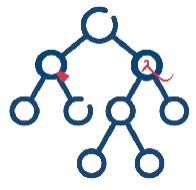
\includegraphics[height=1.0cm]{msca_logo.png}}%
    \end{center}

    \vspace{0.6cm}

    % Main title with Q logos on sides (with clickable links)
    \begin{center}
        \begin{minipage}{0.1\textwidth}
            \centering
            \href{https://quantlet.com}{
\includegraphics[height=1.1cm]{ql_logo.png}}
        \end{minipage}%
        \begin{minipage}{0.78\textwidth}
            \centering
            {\LARGE\bfseries\usebeamercolor[fg]{title}\inserttitle}

            \vspace{0.3cm}

            {\usebeamerfont{subtitle}\usebeamercolor[fg]{title}\insertsubtitle}
        \end{minipage}%
        \begin{minipage}{0.1\textwidth}
            \centering
            \href{https://quantinar.com}{
\includegraphics[height=1.1cm]{qr_logo.png}}
        \end{minipage}
    \end{center}

    \vspace{0.6cm}

    % Authors (left aligned)
    \hspace{0.5cm}{\usebeamerfont{author}\insertauthor}

    \vspace{0.3cm}

    % Institute/Affiliations (left aligned)
    \hspace{0.5cm}\begin{minipage}[t]{0.9\textwidth}
        \raggedright\small\insertinstitute
    \end{minipage}
}

%=============================================================================
% THEOREM ENVIRONMENTS
%=============================================================================
\theoremstyle{definition}
\setbeamertemplate{theorems}[numbered]
\ifdefined\sfmlang
\newtheorem{defn}{Definiție}
\newtheorem{thm}{Teoremă}
\newtheorem{prop}{Propoziție}
\newtheorem{rmk}{Observație}
\else
\newtheorem{defn}{Definition}
\newtheorem{thm}{Theorem}
\newtheorem{prop}{Proposition}
\newtheorem{rmk}{Remark}
\fi

%=============================================================================
% CENTRED MINIPAGE (no extra vertical space)
%=============================================================================
\newenvironment{cminipage}[1]{%
    \par\noindent\hfill\begin{minipage}{#1}\ignorespaces
}{%
    \end{minipage}\hfill\null\par
}

%=============================================================================
% CUSTOM COMMANDS
%=============================================================================
\newcommand{\E}{\mathbb{E}}
\newcommand{\Var}{\text{Var}}
\newcommand{\Cov}{\text{Cov}}
\newcommand{\Corr}{\text{Corr}}
\newcommand{\R}{\mathbb{R}}
\newcommand{\N}{\mathbb{N}}
\newcommand{\Z}{\mathbb{Z}}
\newcommand{\B}{\mathbf{B}}
\newcommand{\imark}{\textcolor{MainBlue}{\textbullet}}
\newcommand{\RMSE}{\text{RMSE}}
\newcommand{\MAE}{\text{MAE}}
\newcommand{\MAPE}{\text{MAPE}}



\newcommand{\qlurl}[1]{https://github.com/danpele/SFM/tree/main/Quantlets/Ch_14/#1}
\renewcommand{\nb}{\colaburl{notebooks/EN/chapter14_seminar_notebook.ipynb}}
\renewcommand{\nbname}{chapter14\_seminar\_notebook.ipynb}
% left column: full width in the student version, narrower next to the solution
\newcommand{\taskw}{\ifsolutions 0.47\textwidth\else 0.96\textwidth\fi}
\newcommand{\solw}{\ifsolutions 0.49\textwidth\else 0pt\fi}

% Clickable citations (DOIs verified via Crossref)

\newcommand{\refNakamoto}{\href{https://bitcoin.org/bitcoin.pdf}{Nakamoto (2008)}}
\newcommand{\refButerin}{\href{https://ethereum.org/en/whitepaper/}{Buterin (2014)}}
\newcommand{\refMerge}{\href{https://ethereum.org/en/roadmap/merge/}{ethereum.org: The Merge}}
\newcommand{\refLT}{\href{https://doi.org/10.1093/rfs/hhaa113}{Liu \& Tsyvinski (2021)}}
\newcommand{\refLTW}{\href{https://doi.org/10.1111/jofi.13119}{Liu, Tsyvinski \& Wu (2022)}}
\newcommand{\refGS}{\href{https://doi.org/10.1111/jofi.12903}{Griffin \& Shams (2020)}}
\newcommand{\refMS}{\href{https://doi.org/10.1016/j.jfineco.2019.07.001}{Makarov \& Schoar (2020)}}
\newcommand{\refGorton}{\href{https://doi.org/10.3386/w30796}{Gorton et al.\ (2022)}}
\newcommand{\refGZ}{\href{https://doi.org/10.2139/ssrn.3888752}{Gorton \& Zhang (2021)}}
\newcommand{\refLVN}{\href{https://doi.org/10.1016/j.jimonfin.2022.102777}{Lyons \& Viswanath-Natraj (2023)}}
\newcommand{\refLMS}{\href{https://doi.org/10.3386/w31160}{Liu, Makarov \& Schoar (2023)}}
\newcommand{\refMZZ}{\href{https://doi.org/10.3386/w33882}{Ma, Zeng \& Zhang (2025)}}
\newcommand{\refUrquhart}{\href{https://doi.org/10.1016/j.econlet.2016.09.019}{Urquhart (2016)}}
\newcommand{\refNC}{\href{https://doi.org/10.1016/j.econlet.2016.10.033}{Nadarajah \& Chu (2017)}}
\newcommand{\refTL}{\href{https://doi.org/10.1016/j.frl.2019.101382}{Tran \& Leirvik (2020)}}
\newcommand{\refCF}{\href{https://doi.org/10.1016/j.econlet.2015.02.029}{Cheah \& Fry (2015)}}
\newcommand{\refKatsiampa}{\href{https://doi.org/10.1016/j.econlet.2017.06.023}{Katsiampa (2017)}}
\newcommand{\refBL}{\href{https://doi.org/10.1111/j.1540-6288.2010.00244.x}{Baur \& Lucey (2010)}}
\newcommand{\refBHL}{\href{https://doi.org/10.1016/j.intfin.2017.12.004}{Baur, Hong \& Lee (2018)}}
\newcommand{\refCP}{\href{https://doi.org/10.1016/j.frl.2018.11.012}{Caporale \& Plastun (2019)}}
\newcommand{\refGHMO}{\href{https://doi.org/10.1016/j.jmoneco.2017.12.004}{Gandal et al.\ (2018)}}
\newcommand{\refHill}{\href{https://doi.org/10.1214/aos/1176343247}{Hill (1975)}}
\newcommand{\refBoll}{\href{https://doi.org/10.1016/0304-4076(86)90063-1}{Bollerslev (1986)}}
\newcommand{\refLM}{\href{https://doi.org/10.1093/rfs/1.1.41}{Lo \& MacKinlay (1988)}}
\newcommand{\refFama}{\href{https://doi.org/10.2307/2325486}{Fama (1970)}}
\newcommand{\refJLS}{\href{https://doi.org/10.1142/S0219024900000115}{Johansen, Ledoit \& Sornette (2000)}}
\newcommand{\refTH}{\href{https://doi.org/10.1016/j.jempfin.2018.08.004}{Trimborn \& Härdle (2018)}}
\newcommand{\refHHR}{\href{https://doi.org/10.1093/jjfinec/nbz033}{Härdle, Harvey \& Reule (2020)}}
\newcommand{\refFHH}{\href{https://doi.org/10.1007/978-3-030-13751-9}{Franke, Härdle \& Hafner (2019)}}
\newcommand{\refKupiec}{\href{https://doi.org/10.3905/jod.1995.407942}{Kupiec (1995)}}
\newcommand{\refWang}{\href{https://doi.org/10.1038/s41586-023-06221-2}{Wang et al.\ (2023)}}
\newcommand{\refPeleA}{\href{https://doi.org/10.1080/1351847X.2021.1960403}{Pele et al.\ (2023)}}
\newcommand{\refPeleB}{\href{https://doi.org/10.3390/e21020102}{Pele \& Mazurencu-Marinescu-Pele (2019)}}
\newcommand{\refMiCA}{\href{https://eur-lex.europa.eu/eli/reg/2023/1114/oj}{Regulamentul (EU) 2023/1114 (MiCA)}}
\newcommand{\refESMA}{\href{https://www.esma.europa.eu/esmas-activities/digital-finance-and-innovation/markets-crypto-assets-regulation-mica}{ESMA: MiCA}}
\newcommand{\refGENIUS}{\href{https://www.govinfo.gov/app/details/PLAW-119publ27}{GENIUS Act, Public Law 119-27}}
\newcommand{\refSEC}{\href{https://www.sec.gov/newsroom/speeches-statements/gensler-statement-spot-bitcoin-011023}{SEC (2024)}}
\newcommand{\refFed}{\href{https://www.federalreserve.gov/newsevents/pressreleases/monetary20230312b.htm}{Trezoreria SUA, Rezerva Federală și FDIC (2023)}}
\newcommand{\refFDIC}{\href{https://www.fdic.gov/news/press-releases/2023/pr23016.html}{FDIC (2023)}}
\newcommand{\refDL}{\href{https://api-docs.defillama.com/}{DefiLlama}}

\title[Statistica piețelor financiare]{Statistica piețelor financiare}
\subtitle{Seminarul 14: Active cripto\ifsolutions\ (versiunea profesorului)\fi}
\author[D.T. Pele]{Daniel Traian PELE}
\institute{Academia de Studii Economice din București\\
IDA Institute Digital Assets\\
Blockchain Research Center\\
AI4EFin Artificial Intelligence for Energy Finance\\
Academia Română, Institutul de Prognoză Economică\\
MSCA Digital Finance}
\date{}

%=============================================================================
\providecommand{\sfmapplink}[3]{\hypertarget{#2}{}\hyperlink{#1}{\beamergotobutton{#3}}}  % APPLINKS-MACROS
\providecommand{\sfmappback}[2]{\begin{tikzpicture}[remember picture,overlay]\node[anchor=south east] at ([xshift=-3mm,yshift=7mm]current page.south east){\hyperlink{#1}{\beamerreturnbutton{#2}}};\end{tikzpicture}}  % APPLINKS-MACROS
\providecommand{\sfmchlink}[2]{\href{#1}{#2}}  % APPLINKS-MACROS
\providecommand{\sfmchlinkt}[2]{\href{#1}{\usebeamercolor[fg]{frametitle}#2}}  % APPLINKS-MACROS
\begin{document}
%=============================================================================

{
\setbeamertemplate{headline}{}
\setbeamertemplate{footline}{}
\begin{frame}[noframenumbering]
    \titlepage
\end{frame}
}
% BEGIN-ACRONYMS (generat de latex/acronyms.py; nu editati manual)
\begin{frame}{Acronime folosite în acest material}
\setbeamertemplate{itemize/enumerate body begin}{\tiny}
\begin{columns}[T]
\begin{column}{0.49\textwidth}
\begin{itemize}\setlength{\itemsep}{0pt}
    \item \textbf{AI}: Artificial Intelligence (inteligență artificială)
    \item \textbf{AR}: AutoRegressive (model); in event studies: Abnormal Return (model autoregresiv; în studiile de eveniment: randament anormal)
    \item \textbf{CI}: Confidence Interval (interval de încredere)
    \item \textbf{COVID-19}: COronaVIrus Disease 2019 (boala provocată de coronavirus, 2019)
    \item \textbf{DAI}: Dai (stablecoin of the MakerDAO protocol) — stablecoin garantat cu active cripto, al protocolului MakerDAO
    \item \textbf{EODHD}: EOD Historical Data (market-data provider) — furnizor de date de piață
    \item \textbf{ES}: Expected Shortfall (pierderea așteptată în coadă)
    \item \textbf{ETF}: Exchange-Traded Fund (fond tranzacționat la bursă)
    \item \textbf{FTX}: FTX Trading Ltd. (crypto exchange, bankrupt in November 2022) — bursa cripto FTX, falimentară în noiembrie 2022
    \item \textbf{GARCH}: Generalised AutoRegressive Conditional Heteroskedasticity (heteroscedasticitate condiționată autoregresivă generalizată)
    \item \textbf{HS}: Historical Simulation (simularea istorică)
    \item \textbf{LR}: Likelihood Ratio (raportul de verosimilitate)
    \item \textbf{LUNA}: Luna (token of the Terra blockchain) — token-ul blockchain-ului Terra
\end{itemize}
\end{column}
\begin{column}{0.49\textwidth}
\begin{itemize}\setlength{\itemsep}{0pt}
    \item \textbf{SUA}: Statele Unite ale Americii
    \item \textbf{SVB}: Silicon Valley Bank (banca Silicon Valley Bank)
    \item \textbf{USDC}: USD Coin (stablecoin garantat cu dolari, emis de Circle)
    \item \textbf{UST}: TerraUSD (stablecoin algoritmic al rețelei Terra)
\end{itemize}
\end{column}
\end{columns}
\end{frame}
% END-ACRONYMS

\begin{frame}{Întrebarea de azi și traseul}
\itemsize{\small}
\begin{itemize}
    \item \textbf{Întrebarea}: cît de riscantă este o poziție cripto și cît de stabil este un stablecoin?
    \begin{itemize}
        \item seminarul are loc \textbf{înaintea} Cursului 14: secțiunea „Noțiuni necesare azi” dă toate definițiile folosite în cerințe
    \end{itemize}
    \item Traseul
    \begin{itemize}
        \item Partea A: anualizarea cu 365 de zile, drawdown-uri, abateri de la paritate în puncte de bază, VaR al unei poziții cripto, pe hîrtie
        \item Partea B: cozile, corelația cu acțiunile, paritatea USDC și backtesting-ul VaR pentru Bitcoin, pe date reale, fiecare cu o întrebare de interpretare
        \item Partea C: o întrebare deschisă pentru proiect și un răspuns AI de verificat
    \end{itemize}
    \item Notebook-ul de azi: \href{\nb}{deschideți notebook-ul seminarului în Google Colab}; fiecare cerință indică secțiunea din notebook
    \item Seminarul are rol de exercițiu și nu se notează; rezolvările cerințelor [Propus] se discută la seminar
\end{itemize}
\end{frame}

\begin{frame}{Harta exercițiilor}
\itemsize{\footnotesize}
\begin{center}
\scriptsize
\begin{tabular}{>{\raggedright\arraybackslash}p{1.1cm}>{\raggedright\arraybackslash}p{7.5cm}>{\raggedright\arraybackslash}p{1.9cm}>{\raggedright\arraybackslash}p{1.4cm}}
\toprule
\textbf{Cerința} & \textbf{Întrebarea} & \textbf{Tipul} & \textbf{Model} \\
\midrule
A1, A2 & anualizarea unei serii cripto cu 365 și cu 252 de zile & Rezolvat, Propus & A1 \\
A3, A4 & drawdown-ul maxim al unei traiectorii de preț și cîștigul necesar pentru recuperare & Rezolvat, Propus & A3 \\
A5, A6 & abaterile de la paritate ale USDC și DAI în martie 2023, în puncte de bază & Rezolvat, Propus & A5 \\
A7, A8 & VaR 1\% și ES 2,5\% ale unei poziții în Bitcoin și în Ethereum & Rezolvat, Propus & A7 \\
B1, B2 & momente, anualizare și indicele de coadă: Bitcoin și S\&P 500; Ethereum și Solana & Rezolvat, Propus & B1 \\
B3, B4 & corelația în perioade calme și de criză: Bitcoin și S\&P 500; Bitcoin și aur, Ethereum și S\&P 500 & Rezolvat, Propus & B3 \\
B5, B6 & paritatea USDC; USDT și DAI & Rezolvat, Propus & B5 \\
B7, B8 & VaR, ES și backtesting: Bitcoin; Ethereum & Rezolvat, Propus & B7 \\
C1, C2 & au schimbat ETF-urile spot comportamentul Bitcoin? ce este greșit într-un răspuns AI? & Propus & B1, B3 \\
\bottomrule
\end{tabular}
\end{center}
\begin{itemize}
    \item \textbf{[Rezolvat]}: rezolvarea completă în slide-uri și în notebook, un model de urmat; \textbf{[Propus]}: îl rezolvați voi, după model
\end{itemize}
\end{frame}

\begin{frame}{Datele folosite}
\itemsize{\small}
\begin{center}
\footnotesize
\begin{tabular}{llll}
\toprule
\textbf{Seria} & \textbf{Sursa} & \textbf{Prețul folosit} & \textbf{Perioada} \\
\midrule
Bitcoin, Ethereum, Solana & EODHD & închidere, 7 zile pe săptămînă & 2014/2016/2020--2026 \\
USDT, USDC, DAI & EODHD & închidere și minimul zilei & 2021--2026 \\
S\&P 500, aur (XAU/USD) & EODHD & închidere, zile lucrătoare & 2014--2026 \\
\bottomrule
\end{tabular}
\end{center}
\begin{itemize}
    \item Randamente logaritmice zilnice în \%: $r_t = 100\,(\ln P_t - \ln P_{t-1})$, fiecare serie pe propriul calendar; ultima zi este 18 septembrie 2026
    \item Două serii împreună: întîi unim prețurile în zilele comune, apoi calculăm randamentele
    \item În notebook: \texttt{returns('btc')}, \texttt{joint\_returns('btc', 'sp500')}, \texttt{describe(k)}, \texttt{peg\_stats('usdc')}; nu este nevoie de cont sau de cheie
\end{itemize}
\end{frame}


%=============================================================================
\section{Noțiuni necesare azi}
%=============================================================================

\begin{frame}{Noțiuni necesare azi (1/4): activele cripto și anualizarea}
\itemsize{\small}
\begin{itemize}
    \item \textbf{Activ cripto}: un activ digital a cărui proprietate este înregistrată într-un \textbf{blockchain}, un lanț public de blocuri de tranzacții
    \begin{itemize}
        \item Bitcoin (2009): ofertă fixă de 21 de milioane de monede; Ethereum (2015): execută programe (contracte inteligente)
        \item tranzacționate pe \textbf{exchange-uri} (platforme de tranzacționare) 24 de ore din 24, 7 zile pe săptămînă
    \end{itemize}
    \item \textbf{Anualizarea} cu $m$ observații pe an (randamente i.i.d.): media $m\,\bar r$, volatilitatea $\sqrt{m}\,s$
    \begin{itemize}
        \item cripto: $m = 365$, $\sqrt{365} = 19{,}105$; acțiuni: $m = 252$, $\sqrt{252} = 15{,}875$
        \item \textbf{Raportul Sharpe} (rata fără risc 0): media anuală / volatilitatea anuală $= \sqrt{m}\,\bar r/s$
    \end{itemize}
    \item Indicele de coadă Hill (\sfmchlink{https://danpele.github.io/SFM/RO/Cursuri/capitol5_cozi_groase_evt.pdf}{Capitolul 5}): $\hat\alpha = [\frac1k\sum_{i \le k}\ln(X_{(i)}/X_{(k+1)})]^{-1}$ pe cele mai mari $k$ pierderi; CI 95\% $\hat\alpha(1 \pm 1{,}96/\sqrt{k})$; $\alpha$ mai mic, coadă mai groasă
\end{itemize}
\end{frame}

\begin{frame}{Noțiuni necesare azi (2/4): drawdown și corelație}
\itemsize{\small}
\begin{itemize}
    \item \textbf{Drawdown}: $D_t = P_t/M_t - 1$, $M_t = \max_{s \le t} P_s$ maximul curent (ultimul maxim istoric)
    \begin{itemize}
        \item \textbf{drawdown maxim} $= \min_t D_t$; pentru a recupera o pierdere $d$, prețul trebuie să crească cu $d/(1 - d)$
    \end{itemize}
    \item \textbf{Corelația} a două serii cu calendare diferite: unim prețurile în zilele comune, apoi calculăm randamentele logaritmice
    \begin{itemize}
        \item transformarea Fisher: $z = \tanh^{-1}(\hat\rho)$ este aproximativ $N(\tanh^{-1}\rho, 1/(n - 3))$; CI 95\%: $\tanh(z \pm 1{,}96/\sqrt{n - 3})$
        \item două perioade independente: $(z_2 - z_1)/\sqrt{1/(n_1 - 3) + 1/(n_2 - 3)} \sim N(0, 1)$ dacă $\rho_1 = \rho_2$
    \end{itemize}
    \item \textbf{Activ de refugiu} (safe haven) \refBL: un activ care nu scade (sau crește) cînd bursa se prăbușește
\end{itemize}
\end{frame}

\begin{frame}{Noțiuni necesare azi (3/4): stablecoins și puncte de bază}
\itemsize{\small}
\begin{itemize}
    \item \textbf{Stablecoin}: un activ cripto conceput să se tranzacționeze la un preț fix, de obicei 1 USD (\textbf{paritatea}, peg)
    \begin{itemize}
        \item garantat fiat (USDT, USDC: rezerve în dolari), garantat cripto (DAI: garanții cripto), algoritmic (UST: fără rezerve, prăbușit în mai 2022)
        \item \textbf{depeg}: prețul se îndepărtează de paritate; martie 2023: a intrat în faliment Silicon Valley Bank (SVB), care deținea o parte din rezervele USDC
    \end{itemize}
    \item \textbf{Punct de bază} (bp) $= 0{,}01\% = 0{,}0001$; \textbf{abaterea de la paritate} $d_t = 10\,000\,(P_t - 1)$ bp
    \begin{itemize}
        \item un deținător care vinde $Q$ monede la prețul $P < 1$ pierde $Q(1 - P)$ dolari
    \end{itemize}
    \item \textbf{AR(1)} pentru abatere: $d_t = c + \phi\,d_{t-1} + e_t$, $|\phi| < 1$
    \begin{itemize}
        \item \textbf{timpul de înjumătățire} $\ln 0{,}5/\ln\phi$: numărul de zile după care dispare jumătate din abatere
    \end{itemize}
\end{itemize}
\end{frame}

\begin{frame}{Noțiuni necesare azi (4/4): VaR, ES și backtesting}
\itemsize{\footnotesize}
\begin{itemize}
    \item $\mathrm{VaR}_\alpha = -q_\alpha$: pierderea depășită cu probabilitatea $\alpha$ (\textbf{VaR 1\%}); $\mathrm{ES}_\alpha = -E[r \mid r \le q_\alpha]$ (\textbf{ES 2,5\%})
    \begin{itemize}
        \item distribuția Normală: $\mathrm{VaR}_{1\%} = -\mu + 2{,}326\,\sigma$, $\mathrm{ES}_{2,5\%} = -\mu + \sigma\varphi(1{,}960)/0{,}025$, $\varphi(1{,}960) = 0{,}0584$
        \item simularea istorică: $k = \lceil n\alpha\rceil$, VaR $= -r_{(k)}$, ES $= -$ media celor mai mici $k$ randamente
    \end{itemize}
    \item În bani: pentru randamente simple $W \times \mathrm{VaR}/100$; pentru randamente logaritmice $W(1 - e^{-\mathrm{VaR}/100})$
    \begin{itemize}
        \item $h$ zile (i.i.d., media 0): $\sqrt{h}\,\mathrm{VaR}$; cripto: $h$ zile calendaristice
    \end{itemize}
    \item \textbf{Backtesting} \refKupiec: $x$ depășiri ($r_t < -\mathrm{VaR}_t$) în $n$ zile; $LR = -2[\ln L(0{,}01) - \ln L(x/n)] \sim \chi^2(1)$, valoarea critică 3,84
    \begin{itemize}
        \item GARCH(1,1)-t (\sfmchlink{https://danpele.github.io/SFM/RO/Cursuri/capitol9_modele_arch_garch.pdf}{Capitolul 9}): $\sigma_t^2 = \omega + \alpha\varepsilon_{t-1}^2 + \beta\sigma_{t-1}^2$; VaR pentru mîine $= -(\mu + \sigma_{t+1}q_{1\%})$
    \end{itemize}
\end{itemize}
\end{frame}


%=============================================================================
\section{Partea A: calcule pe hîrtie}
%=============================================================================

\begin{frame}{A1: anualizarea Bitcoin [Rezolvat]}
\itemsize{\scriptsize}
\begin{columns}[T]
\begin{column}{0.47\textwidth}
\begin{block}{Cerință}
\begin{itemize}
    \item Randamentele logaritmice zilnice ale Bitcoin: media $\bar r = 0{,}12\%$, abaterea standard $s = 3{,}5\%$. Un analist folosește convenția de la acțiuni, cu 252 de zile.
    \item 1. Calculați media și volatilitatea anuale cu 365 de zile.
    \item 2. Calculați-le cu 252 de zile și precizați cu cît sînt subestimate.
    \item 3. Calculați raportul Sharpe (rata fără risc 0) corect și cu media $\times 252$ și volatilitatea $\times\sqrt{365}$.
    \item Raportați: șase valori și o frază.
\end{itemize}
\end{block}
\end{column}
\begin{column}{0.49\textwidth}
\begin{exampleblock}{Rezolvare}
\begin{itemize}
    \item 1. $365 \times 0{,}12 = 43{,}8\%$; $\sqrt{365} \times 3{,}5 = 19{,}10 \times 3{,}5 = 66{,}9\%$
    \item 2. $252 \times 0{,}12 = 30{,}2\%$ (o subestimare de 31{,}0\%); $\sqrt{252} \times 3{,}5 = 55{,}6\%$ (o subestimare de 16{,}9\%)
    \item 3. Corect: $43{,}8/66{,}9 = 0{,}66$; amestecat: $30{,}2/66{,}9 = 0{,}45$
    \item Convenția cu 252 de zile face ca Bitcoin să pară mai liniștit; amestecul convențiilor îl face să pară mai prost.
\end{itemize}
\end{exampleblock}
\end{column}
\end{columns}
\end{frame}

\begin{frame}{A2: anualizarea Ethereum [Propus]}
\propsub
\itemsize{\scriptsize}
\begin{columns}[T]
\begin{column}{\taskw}
\begin{block}{Cerință}
\begin{itemize}
    \item Randamentele logaritmice zilnice ale Ethereum: $\bar r = 0{,}20\%$, $s = 5{,}0\%$. Model: A1.
    \item 1. Calculați media și volatilitatea anuale cu 365 și cu 252 de zile.
    \item 2. Calculați raportul celor două volatilități.
    \item 3. Calculați raportul Sharpe corect și pe cel amestecat.
    \item Raportați: șapte valori și o frază.
\end{itemize}
\end{block}
\end{column}
\begin{column}{\solw}
\solonly{%
\begin{exampleblock}{Rezolvare}
\begin{itemize}
    \item 1. Media: 73{,}0\% (365) și 50{,}4\% (252); volatilitatea: 95{,}5\% și 79{,}4\%
    \item 2. $\sqrt{365/252} = 1{,}204$ pentru orice $s$
    \item 3. Corect $0{,}76$; amestecat $0{,}53$
    \item Subestimarea (16{,}9\% pentru volatilitate) nu depinde de activ, ci doar de convenție.
\end{itemize}
\end{exampleblock}
}
\end{column}
\end{columns}
\end{frame}

\begin{frame}{A3: drawdown-ul maxim al unei traiectorii de preț [Rezolvat]}
\itemsize{\scriptsize}
\begin{columns}[T]
\begin{column}{0.47\textwidth}
\begin{block}{Cerință}
\begin{itemize}
    \item Închideri lunare ale unui activ cripto, în mii USD: 20, 35, 69, 50, 30, 16, 25, 45, 73.
    \item 1. Scrieți maximul curent $M_t$ și drawdown-ul $D_t$ pentru fiecare lună.
    \item 2. Precizați drawdown-ul maxim și cîștigul necesar pentru recuperarea de la minim.
    \item 3. Precizați în ce lună își revine activul.
    \item Raportați: două valori, o listă și o frază.
\end{itemize}
\end{block}
\end{column}
\begin{column}{0.49\textwidth}
\begin{exampleblock}{Rezolvare}
\begin{itemize}
    \item 1. $M_t$: 20; 35; 69; 69; 69; 69; 69; 69; 73; $D_t$ (\%): $0{,}0$; $0{,}0$; $0{,}0$; $-27{,}5$; $-56{,}5$; $-76{,}8$; $-63{,}8$; $-34{,}8$; $0{,}0$
    \item 2. Drawdown-ul maxim $16/69 - 1 = -76{,}8\%$; cîștigul necesar $69/16 - 1 = 331{,}25\%$
    \item 3. Luna 9 (73 $>$ 69): un nou maxim istoric.
    \item O scădere de aproximativ trei sferturi cere mai mult decît o cvadruplare pentru recuperare.
\end{itemize}
\end{exampleblock}
\end{column}
\end{columns}
\end{frame}

\begin{frame}{A4: o a doua traiectorie de preț [Propus]}
\propsub
\itemsize{\scriptsize}
\begin{columns}[T]
\begin{column}{\taskw}
\begin{block}{Cerință}
\begin{itemize}
    \item Închideri trimestriale ale Ethereum, în mii USD: 1,4; 4,8; 3,2; 0,9; 1,2; 2,5; 4,9. Model: A3.
    \item 1. Scrieți maximul curent și drawdown-urile.
    \item 2. Precizați drawdown-ul maxim și cîștigul necesar pentru recuperare.
    \item 3. Precizați în ce trimestru își revine activul.
    \item Raportați: două valori, o listă și o frază.
\end{itemize}
\end{block}
\end{column}
\begin{column}{\solw}
\solonly{%
\begin{exampleblock}{Rezolvare}
\begin{itemize}
    \item 1. $M_t$: 1{,}4; 4{,}8; 4{,}8; 4{,}8; 4{,}8; 4{,}8; 4{,}9; $D_t$ (\%): $0{,}0$; $0{,}0$; $-33{,}3$; $-81{,}2$; $-75{,}0$; $-47{,}9$; $0{,}0$
    \item 2. $0{,}9/4{,}8 - 1 = -81{,}2\%$; cîștigul necesar $4{,}8/0{,}9 - 1 = 433{,}33\%$
    \item 3. Trimestrul 7.
    \item Cîștigul de recuperare crește repede cu adîncimea: $d/(1 - d)$ explodează cînd $d \to 1$.
\end{itemize}
\end{exampleblock}
}
\end{column}
\end{columns}
\end{frame}

\begin{frame}{A5: USDC în martie 2023 [Rezolvat]}
\itemsize{\scriptsize}
\begin{columns}[T]
\begin{column}{0.47\textwidth}
\begin{block}{Cerință}
\begin{itemize}
    \item Închiderile zilnice USDC: 10 martie 2023 0{,}9995, 11 martie 0{,}9715, 12 martie 0{,}9921, 13 martie 0{,}9989; cel mai mic minim zilnic 0{,}8774 (11 martie).
    \item 1. Calculați abaterea de la paritate a fiecărei închideri în puncte de bază.
    \item 2. Calculați abaterea celui mai mic minim.
    \item 3. Calculați pierderea unui deținător de 1\,000\,000 USDC care a vîndut la cea mai proastă închidere și la cel mai mic minim.
    \item Raportați: cinci abateri, două pierderi și o frază.
\end{itemize}
\end{block}
\end{column}
\begin{column}{0.49\textwidth}
\begin{exampleblock}{Rezolvare}
\begin{itemize}
    \item 1. $10\,000(P - 1)$: $-5$; $-285$; $-79$; $-11$ bp
    \item 2. $10\,000 \times (0{,}8774 - 1) = -1226$ bp
    \item 3. $1\,000\,000 \times (1 - 0{,}9715) = 28\,500$ USD; la minim: 122\,600 USD
    \item Cine a vîndut în panică sîmbătă a pierdut; cine a păstrat moneda pînă luni, după garantarea depozitelor, nu a pierdut aproape nimic.
\end{itemize}
\end{exampleblock}
\end{column}
\end{columns}
\end{frame}

\begin{frame}{A6: DAI în martie 2023 [Propus]}
\propsub
\itemsize{\scriptsize}
\begin{columns}[T]
\begin{column}{\taskw}
\begin{block}{Cerință}
\begin{itemize}
    \item Închiderile zilnice DAI: 10 martie 2023 0{,}9990, 11 martie 0{,}9739, 12 martie 0{,}9926, 13 martie 0{,}9989; cel mai mic minim zilnic 0{,}8970. Model: A5.
    \item 1. Calculați cele patru abateri ale închiderilor și abaterea minimului în bp.
    \item 2. Calculați pierderea pentru 1\,000\,000 DAI vînduți la cea mai proastă închidere și la minim.
    \item 3. Explicați de ce DAI, o monedă garantată cripto, a urmat USDC.
    \item Raportați: cinci abateri, două pierderi și o frază.
\end{itemize}
\end{block}
\end{column}
\begin{column}{\solw}
\solonly{%
\begin{exampleblock}{Rezolvare}
\begin{itemize}
    \item 1. $-10$; $-261$; $-74$; $-11$ bp; minimul $-1030$ bp
    \item 2. 26\,100 USD la închidere; 103\,000 USD la minim
    \item 3. O mare parte din garanția DAI era în USDC: o monedă garantată cripto moștenește riscul garanției ei.
\end{itemize}
\end{exampleblock}
}
\end{column}
\end{columns}
\end{frame}

\begin{frame}{A7: VaR al unei poziții în Bitcoin [Rezolvat]}
\itemsize{\scriptsize}
\begin{columns}[T]
\begin{column}{0.47\textwidth}
\begin{block}{Cerință}
\begin{itemize}
    \item O poziție de 100\,000 USD în Bitcoin.
    \item 1. Cu randamente zilnice simple Normale ($\mu = 0{,}10\%$, $\sigma = 3{,}5\%$), calculați VaR 1\%, ES 2,5\% și VaR 1\% pe 10 zile, în \% și în USD.
    \item 2. Cele mai mici 10 din ultimele 365 de randamente logaritmice (19 septembrie 2025 -- 18 septembrie 2026), în \%: $-15{,}23$; $-7{,}23$; $-6{,}77$; $-6{,}69$; $-5{,}46$; $-5{,}43$; $-5{,}32$; $-4{,}76$; $-4{,}69$; $-4{,}62$. Calculați VaR 1\% și ES 2,5\% istorice, în \% și în USD.
    \item Raportați: zece valori și o frază.
\end{itemize}
\end{block}
\end{column}
\begin{column}{0.49\textwidth}
\begin{exampleblock}{Rezolvare}
\begin{itemize}
    \item 1. VaR $= -0{,}10 + 2{,}326 \times 3{,}5 = 8{,}04\%$ (8\,042 USD); ES $= -0{,}10 + 3{,}5 \times 0{,}0584/0{,}025 = 8{,}08\%$ (8\,082 USD); 10 zile: $\sqrt{10} \times 2{,}326 \times 3{,}5 = 25{,}75\%$ (25\,748 USD)
    \item 2. $k = \lceil 3{,}65 \rceil = 4$: VaR 1\% $= 6{,}69\%$, $100\,000(1 - 0{,}9353) = 6\,471$ USD; $k = \lceil 9{,}125 \rceil = 10$: ES 2,5\% $= 66{,}20/10 = 6{,}62\%$ (6\,406 USD)
    \item ES 2,5\% poate fi sub VaR 1\%: ES $\ge$ VaR este valabilă doar la același nivel.
\end{itemize}
\end{exampleblock}
\end{column}
\end{columns}
\end{frame}

\begin{frame}{A8: VaR al unei poziții în Ethereum [Propus]}
\propsub
\itemsize{\scriptsize}
\begin{columns}[T]
\begin{column}{\taskw}
\begin{block}{Cerință}
\begin{itemize}
    \item O poziție de 100\,000 USD în Ethereum. Model: A7.
    \item 1. Cu randamente simple Normale ($\mu = 0{,}20\%$, $\sigma = 5{,}0\%$), calculați VaR 1\%, ES 2,5\% și VaR 1\% pe 10 zile, în \% și în USD.
    \item 2. Cele mai mici 10 din ultimele 365 de randamente logaritmice, în \%: $-16{,}27$; $-12{,}83$; $-11{,}28$; $-10{,}00$; $-8{,}99$; $-8{,}22$; $-8{,}20$; $-7{,}54$; $-7{,}52$; $-7{,}11$. Calculați VaR 1\% și ES 2,5\% istorice, în \% și în USD.
    \item Raportați: zece valori și o frază.
\end{itemize}
\end{block}
\end{column}
\begin{column}{\solw}
\solonly{%
\begin{exampleblock}{Rezolvare}
\begin{itemize}
    \item 1. VaR 11{,}43\% (11\,432 USD); ES 11{,}49\% (11\,489 USD); 10 zile 36{,}78\% (36\,783 USD)
    \item 2. VaR 1\% $= 10{,}00\%$ (9\,516 USD); ES 2,5\% $= 97{,}96/10 = 9{,}80\%$ (9\,331 USD)
    \item Ultimul an a fost mai liniștit decît presupune modelul Normal cu $\sigma = 5\%$.
\end{itemize}
\end{exampleblock}
}
\end{column}
\end{columns}
\end{frame}


%=============================================================================
\section{Partea B: date reale, inferență și interpretare}
%=============================================================================

\begin{frame}{B1: Bitcoin comparat cu S\&P 500 [Rezolvat]}
\itemsize{\footnotesize}
\begin{itemize}
\item \textbf{Întrebarea}: diferă distribuția Bitcoin de cea a S\&P 500 doar prin scală sau și prin forma cozilor?
\item \textbf{Date}: închiderile Bitcoin și S\&P 500 din septembrie 2014, randamente logaritmice zilnice în \%, fiecare pe propriul calendar
\item \textbf{Cerințe}
\begin{enumerate}
    \item Calculați media, abaterea standard, asimetria și excesul de boltire pentru fiecare serie.
    \item Anualizați media și volatilitatea cu frecvența reală și cu 252 de zile.
    \item Calculați indicele Hill pentru coada stîngă și pentru coada dreaptă cu $k = 2{,}5\%$ din $n$ și intervalul de încredere de 95\%.
    \item Desenați graficul Hill al pierderilor pentru ambele serii.
    \item Interpretare: are Bitcoin cozi mai groase decît S\&P 500?
\end{enumerate}
\item \textbf{Raportați}: un tabel cu 12 valori, graficul și două fraze
\item Notebook: secțiunea B1
\end{itemize}
\end{frame}

\begin{frame}{B1: rezolvare [Rezolvat]}
\itemsize{\scriptsize}
\begin{center}
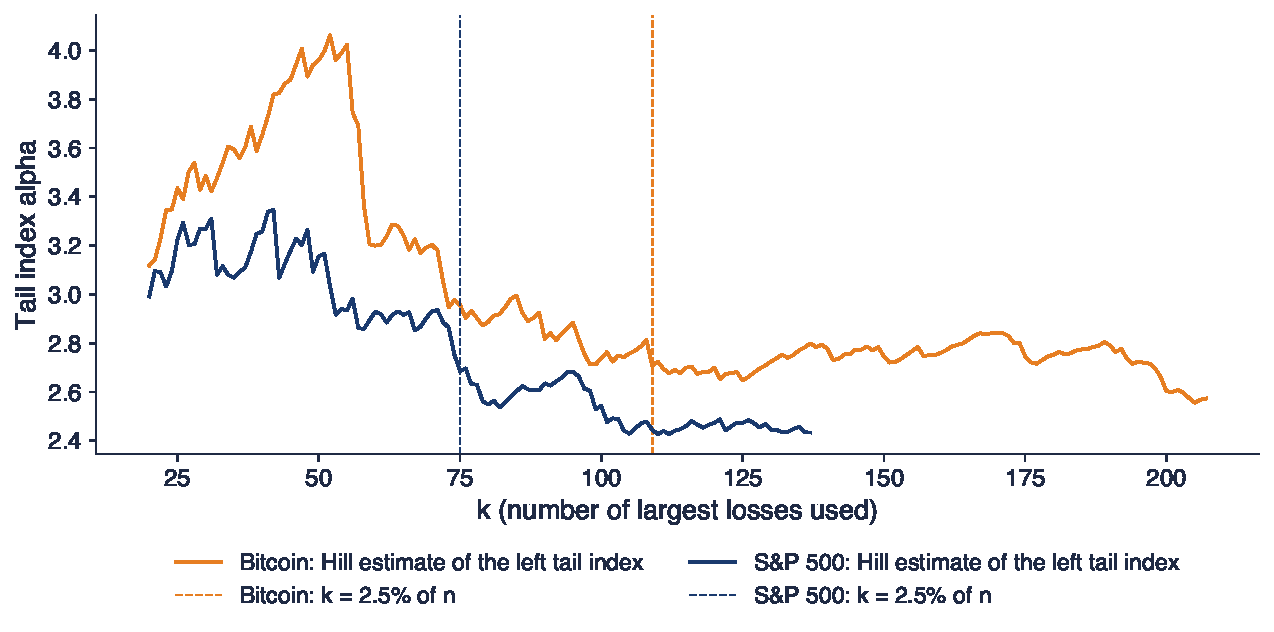
\includegraphics[width=0.96\textwidth,height=0.30\textheight,keepaspectratio]{ch14_sem_b1.pdf}
\end{center}
\vspace{-2mm}
\begin{center}
\scriptsize
\begin{tabular}{lrrrrrrrr}
\toprule
& $n$ & ab.\ std. & asim. & exces boltire & vol.\ ($m$ real) & vol.\ (252) & $\hat\alpha$ stînga [CI 95\%] & $\hat\alpha$ dreapta \\
\midrule
Bitcoin & 4\,384 & $3{,}49$ & $-0{,}70$ & $12{,}0$ & $66{,}6$ & $55{,}3$ & $2{,}71$ $[2{,}20; 3{,}21]$ & $3{,}37$ \\
S\&P 500 & 3\,017 & $1{,}11$ & $-0{,}64$ & $15{,}8$ & $17{,}6$ & $17{,}6$ & $2{,}68$ $[2{,}08; 3{,}29]$ & $2{,}80$ \\
\bottomrule
\end{tabular}
\end{center}
\begin{itemize}
    \item Mediile: 0{,}118\% și 0{,}044\% pe zi; mediile anuale 43{,}1\% ($m = 365{,}3$) și 11{,}2\% ($m = 251{,}4$); cu 252 de zile, volatilitatea Bitcoin ar fi 55{,}3\%
    \item Interpretare: nu: indicii cozii stîngi sînt aproape egali, iar intervalele lor se suprapun; Bitcoin este de circa patru ori mai volatil, dar coada lui are aceeași formă: diferența este de scală
\end{itemize}\sfmquantlet{Ch_14}{SFM_ch14_seminar}
\end{frame}

\begin{frame}{B2: Ethereum și Solana [Propus]}
\itemsize{\footnotesize}
\begin{itemize}
\item \textbf{Întrebarea}: se păstrează concluziile din B1 pentru alte două active cripto mari? Model: B1.
\item \textbf{Date}: Ethereum din 2016, Solana din aprilie 2020; randamente logaritmice zilnice în \%
\item \textbf{Cerințe}
\begin{enumerate}
    \item Calculați cele patru momente pentru fiecare serie.
    \item Anualizați volatilitatea cu 365 și cu 252 de zile.
    \item Calculați ambii indici Hill cu intervalele lor de 95\%.
    \item Interpretare: care dintre activele din B1 și B2 are cea mai groasă coadă stîngă?
\end{enumerate}
\item \textbf{Raportați}: un tabel și două fraze
\item Notebook: secțiunea B2
\end{itemize}
\end{frame}

\ifsolutions
\begin{frame}{B2: rezolvare [Propus]}
\itemsize{\footnotesize}
\begin{center}
\scriptsize
\begin{tabular}{lrrrrrrr}
\toprule
& $n$ & ab.\ std. & asim. & exces boltire & vol.\ 365 & vol.\ 252 & $\hat\alpha$ stînga [CI 95\%] \\
\midrule
Ethereum & 3\,913 & $4{,}99$ & $-0{,}20$ & $9{,}0$ & $95{,}3$ & $79{,}2$ & $2{,}62$ $[2{,}10; 3{,}15]$ \\
Solana & 2\,351 & $6{,}12$ & $-0{,}22$ & $7{,}9$ & $117{,}1$ & $97{,}2$ & $2{,}84$ $[2{,}11; 3{,}57]$ \\
\bottomrule
\end{tabular}
\end{center}
\begin{itemize}
    \item Cozile drepte: $\hat\alpha = 3{,}09$ (Ethereum), $3{,}41$ (Solana): coada stîngă este mai groasă, ca la Bitcoin
    \item Interpretare: Ethereum are cea mai mică estimare punctuală ($2{,}62$), dar toate intervalele se suprapun: cu 58--97 de observații în coadă nu putem ordona cele cinci cozi; volatilitățile diferă clar
\end{itemize}\sfmquantlet{Ch_14}{SFM_ch14_seminar}
\end{frame}
\fi

\begin{frame}{B3: Bitcoin și S\&P 500 în perioade calme și de criză [Rezolvat]}
\itemsize{\footnotesize}
\begin{itemize}
\item \textbf{Întrebarea}: s-a schimbat corelația dintre Bitcoin și acțiuni după 2020 și ce s-a întîmplat în crizele din 2020 și 2022?
\item \textbf{Date}: închiderile Bitcoin și S\&P 500 din septembrie 2014, unite în zilele comune; randamente logaritmice zilnice și săptămînale (vineri--vineri)
\item \textbf{Cerințe}
\begin{enumerate}
    \item Calculați corelația înainte de 2020 și din 2020 și testați egalitatea lor cu testul $z$ al lui Fisher.
    \item Calculați corelația randamentelor zilnice și săptămînale an cu an și reprezentați-le grafic.
    \item Calculați randamentele cumulate ale ambelor serii în episoadele COVID-19, Terra/Luna și FTX.
    \item Calculați randamentul mediu al Bitcoin în cele mai proaste 5\% dintre zilele S\&P 500.
    \item Interpretare: diversifică Bitcoin un portofoliu de acțiuni atunci cînd este cea mai mare nevoie?
\end{enumerate}
\item \textbf{Raportați}: șase valori, graficul și două fraze
\item Notebook: secțiunea B3
\end{itemize}
\end{frame}

\begin{frame}{B3: rezolvare [Rezolvat]}
\itemsize{\scriptsize}
\begin{center}
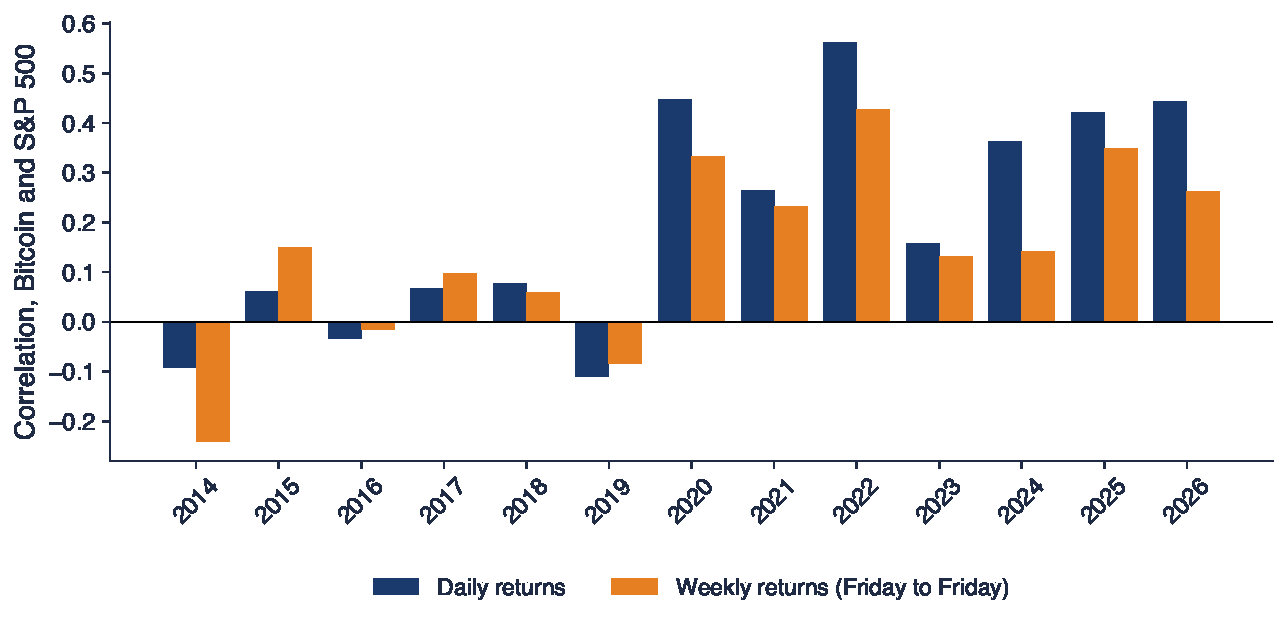
\includegraphics[width=0.96\textwidth,height=0.32\textheight,keepaspectratio]{ch14_sem_b3.pdf}
\end{center}
\vspace{-2mm}
\begin{itemize}
    \item Înainte de 2020: $\hat\rho = 0{,}02$ ($n = 1\,330$); din 2020: $\hat\rho = 0{,}39$, CI 95\% $[0{,}35; 0{,}43]$ ($n = 1\,687$); Fisher $z = 10{,}71$, p $<$\,0{,}001
    \item Randamente logaritmice cumulate (Bitcoin; S\&P 500): COVID-19 $-40{,}6\%$; $-41{,}4\%$; Terra/Luna $-23{,}0\%$; $-5{,}4\%$; FTX $-29{,}9\%$; $4{,}6\%$
    \item În cele 151 de zile cele mai proaste ale S\&P 500 (media $-2{,}70\%$), Bitcoin a avut în medie $-2{,}77\%$; corelația săptămînală pe întreaga perioadă 0{,}19, cea zilnică 0{,}24
    \item Interpretare: nu: din 2020 corelația este semnificativ pozitivă, iar în cele mai proaste zile ale acțiunilor Bitcoin scade cît S\&P 500; crizele specifice cripto (Terra, FTX) nu s-au extins la acțiuni
\end{itemize}\sfmquantlet{Ch_14}{SFM_ch14_seminar}
\end{frame}

\begin{frame}{B4: Bitcoin și aurul, Ethereum și S\&P 500 [Propus]}
\itemsize{\footnotesize}
\begin{itemize}
\item \textbf{Întrebarea}: este Bitcoin legat de aur și se comportă Ethereum ca Bitcoin față de acțiuni? Model: B3.
\item \textbf{Date}: Bitcoin și aurul (XAU/USD) din 2014; Ethereum și S\&P 500 din 2016; prețuri unite în zilele comune
\item \textbf{Cerințe}
\begin{enumerate}
    \item Calculați ambele corelații înainte și după 2020 și testați egalitatea lor.
    \item Calculați corelațiile din 2022 și 2025, zilnice și săptămînale.
    \item Calculați randamentul mediu al Bitcoin în cele mai proaste 5\% dintre zilele aurului și al Ethereum în cele mai proaste 5\% dintre zilele S\&P 500.
    \item Interpretare: este Bitcoin „aur digital”?
\end{enumerate}
\item \textbf{Raportați}: un tabel și două fraze
\item Notebook: secțiunea B4
\end{itemize}
\end{frame}

\ifsolutions
\begin{frame}{B4: rezolvare [Propus]}
\itemsize{\footnotesize}
\begin{center}
\scriptsize
\begin{tabular}{lrrrrrrr}
\toprule
& înainte de 2020 & din 2020 & Fisher $z$ (p) & 2022 z./săpt. & 2025 z./săpt. & media în zilele proaste \\
\midrule
Bitcoin, aur & $-0{,}01$ & $0{,}15$ & $4{,}47$ ($<$\,0{,}001) & $0{,}15$/$0{,}11$ & $0{,}12$/$0{,}00$ & $-0{,}76$ \\
Ethereum, S\&P 500 & $0{,}02$ & $0{,}40$ & $10{,}23$ ($<$\,0{,}001) & $0{,}55$/$0{,}51$ & $0{,}46$/$0{,}33$ & $-4{,}42$ \\
\bottomrule
\end{tabular}
\end{center}
\begin{itemize}
    \item Zilele proaste: cele mai proaste 5\% dintre zilele celei de-a doua serii (aurul; S\&P 500); media primei serii în \%
    \item Interpretare: nu: corelația cu aurul a crescut doar la 0{,}15, iar Bitcoin nu își păstrează valoarea nici cînd scade aurul, nici cînd scad acțiunile; Ethereum se mișcă împreună cu acțiunile chiar mai mult decît Bitcoin
\end{itemize}\sfmquantlet{Ch_14}{SFM_ch14_seminar}
\end{frame}
\fi

\begin{frame}{B5: cît de stabil este USDC? [Rezolvat]}
\itemsize{\footnotesize}
\begin{itemize}
\item \textbf{Întrebarea}: cît de mult și pentru cît timp se îndepărtează USDC de 1 USD?
\item \textbf{Date}: închiderile și minimele zilnice USDC din 1 ianuarie 2021
\item \textbf{Cerințe}
\begin{enumerate}
    \item Calculați abaterile de la paritate în bp, abaterea lor standard și valoarea absolută mediană.
    \item Calculați proporția zilelor din clasele sub 1, 1--5, 5--10, 10--50 și peste 50 bp și reprezentați-le grafic.
    \item Estimați un AR(1) pentru abatere și calculați timpul de înjumătățire al unei abateri.
    \item Comparați abaterea standard dinainte de 2023 cu cea de după aprilie 2023.
    \item Interpretare: poate un trezorier să trateze USDC ca numerar?
\end{enumerate}
\item \textbf{Raportați}: șase valori, graficul și două fraze
\item Notebook: secțiunea B5
\end{itemize}
\end{frame}

\begin{frame}{B5: rezolvare [Rezolvat]}
\itemsize{\scriptsize}
\begin{center}
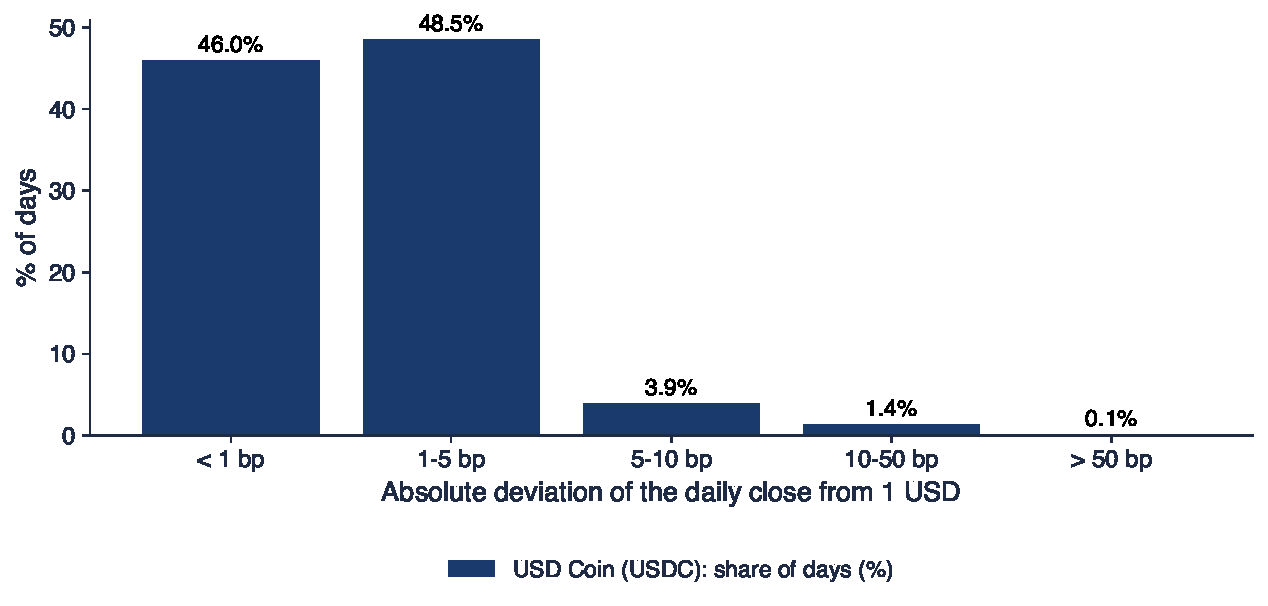
\includegraphics[width=0.96\textwidth,height=0.30\textheight,keepaspectratio]{ch14_sem_b5.pdf}
\end{center}
\vspace{-2mm}
\begin{itemize}
    \item $n = 2\,087$ zile; abaterea standard 7{,}5 bp, $|d_t|$ median 1{,}1 bp; 1{,}5\% din zile peste 10 bp, 0{,}14\% peste 50 bp; cea mai proastă închidere $-285$ bp (11 martie 2023), cel mai prost minim $-1226$ bp
    \item AR(1): $\hat\phi = 0{,}290$ (se $0{,}021$), timpul de înjumătățire 0{,}56 zile; abaterea standard 5{,}8 bp în 2021--2022, 1{,}5 bp după aprilie 2023
    \item Interpretare: aproape întotdeauna: într-o zi obișnuită USDC este la cîțiva bp de paritate, iar abaterile se închid într-o zi; dar coada este reală: într-un weekend din 2023 un deținător putea pierde 3\% la închidere și 12\% la minim
\end{itemize}\sfmquantlet{Ch_14}{SFM_ch14_seminar}
\end{frame}

\begin{frame}{B6: USDT și DAI [Propus]}
\itemsize{\footnotesize}
\begin{itemize}
\item \textbf{Întrebarea}: sînt USDT și DAI la fel de stabile ca USDC? Model: B5.
\item \textbf{Date}: închiderile și minimele zilnice USDT și DAI din 1 ianuarie 2021
\item \textbf{Cerințe}
\begin{enumerate}
    \item Calculați abaterea standard, abaterea absolută mediană și proporțiile peste 10 și 50 bp.
    \item Găsiți cea mai proastă închidere și cel mai prost minim pentru fiecare monedă, cu datele lor.
    \item Estimați AR(1) și calculați timpii de înjumătățire.
    \item Interpretare: care dintre cele trei monede păstrează cel mai bine paritatea în perioade normale și care în criză?
\end{enumerate}
\item \textbf{Raportați}: un tabel și două fraze
\item Notebook: secțiunea B6
\end{itemize}
\end{frame}

\ifsolutions
\begin{frame}{B6: rezolvare [Propus]}
\itemsize{\footnotesize}
\begin{center}
\scriptsize
\begin{tabular}{lrrrrrrr}
\toprule
& ab.\ std. & $|d|$ median & $>$10 bp (\%) & $>$50 bp (\%) & cea mai proastă închidere & cel mai prost minim & înjumătățire \\
\midrule
USDT & $7{,}3$ & $3{,}1$ & $11{,}4$ & $0{,}14$ & $-41$ & $-515$ & $2{,}16$ \\
DAI & $10{,}8$ & $2{,}2$ & $10{,}7$ & $0{,}57$ & $-261$ & $-1030$ & $0{,}63$ \\
USDC & $7{,}5$ & $1{,}1$ & $1{,}5$ & $0{,}14$ & $-285$ & $-1226$ & $0{,}56$ \\
\bottomrule
\end{tabular}
\end{center}
\begin{itemize}
    \item Cele mai proaste închideri: USDT pe 11 mai 2022, DAI pe 11 martie 2023; abaterile în bp, timpii de înjumătățire în zile
    \item Interpretare: în perioade normale USDC este cel mai strîns legat de paritate (mediana 1{,}1 bp), iar USDT cel mai puțin, cu cea mai lentă revenire; în martie 2023 USDT a rămas la paritate, în timp ce USDC și DAI au rupt-o: stabilitatea din perioadele calme spune puțin despre crize
\end{itemize}\sfmquantlet{Ch_14}{SFM_ch14_seminar}
\end{frame}
\fi

\begin{frame}{B7: riscul unei poziții în Bitcoin [Rezolvat]}
\itemsize{\footnotesize}
\begin{itemize}
\item \textbf{Întrebarea}: cît poate pierde într-o zi o poziție de 100\,000 USD în Bitcoin și ce model ar fi trecut un backtesting?
\item \textbf{Date}: închiderile Bitcoin din septembrie 2014, randamente logaritmice zilnice în \%
\item \textbf{Cerințe}
\begin{enumerate}
    \item Calculați VaR 1\% și ES 2,5\% prin simulare istorică, cu distribuția Normală, cu Student-t (verosimilitate maximă) și cu GARCH(1,1)-t pentru ziua următoare.
    \item Convertiți-le în USD cu $W(1 - e^{-v/100})$.
    \item Verificați VaR 1\% pe o zi din 2018: simulare istorică pe ultimele 365 de zile și GARCH(1,1)-t reestimat la fiecare 365 de zile; numărați depășirile și aplicați testul Kupiec.
    \item Interpretare: ce valoare ați raporta unui comitet de risc?
\end{enumerate}
\item \textbf{Raportați}: un tabel cu opt valori, graficul, două rezultate de test și două fraze
\item Notebook: secțiunea B7
\end{itemize}
\end{frame}

\begin{frame}{B7: rezolvare [Rezolvat]}
\itemsize{\scriptsize}
\begin{center}
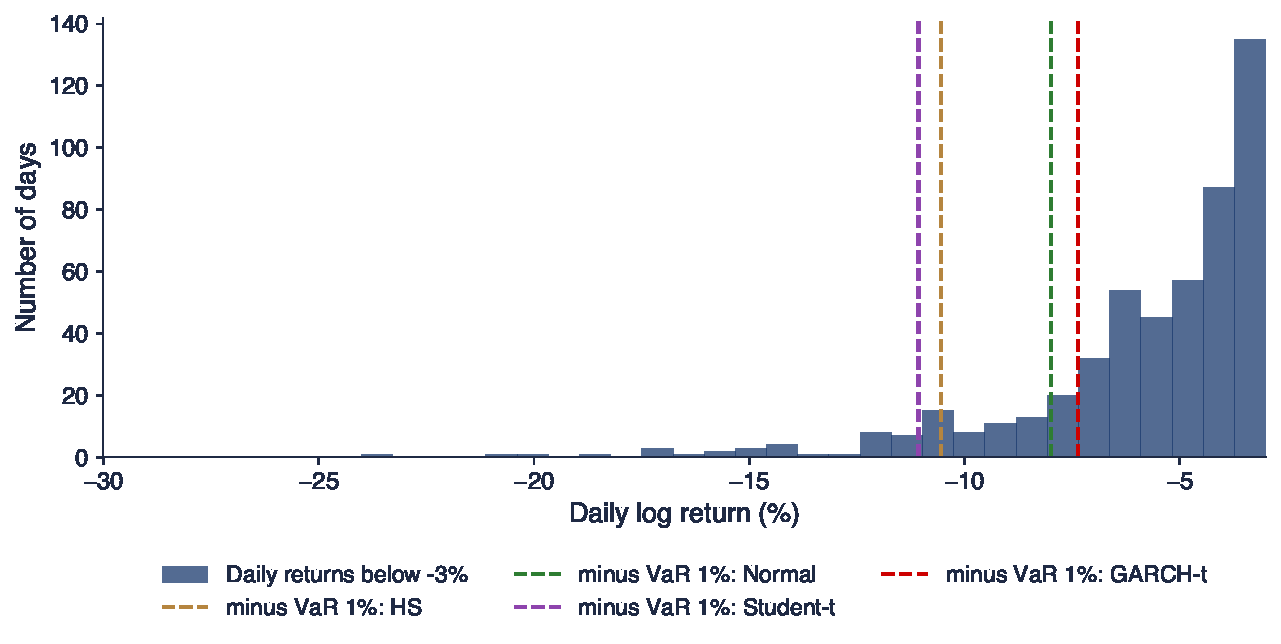
\includegraphics[width=0.96\textwidth,height=0.28\textheight,keepaspectratio]{ch14_sem_b7.pdf}
\end{center}
\vspace{-2mm}
\begin{center}
\scriptsize
\begin{tabular}{lrrrr}
\toprule
& HS & Normală & Student-t & GARCH-t \\
\midrule
VaR 1\% (\%) & $10{,}54$ & $7{,}99$ & $11{,}06$ & $7{,}37$ \\
VaR 1\% (USD) & 10\,006 & 7\,679 & 10\,474 & 7\,105 \\
ES 2,5\% (\%) & $10{,}84$ & $8{,}03$ & $13{,}37$ & $8{,}11$ \\
\bottomrule
\end{tabular}
\end{center}
\begin{itemize}
    \item $n = 4\,384$; Student-t $\hat\nu = 2{,}23$; GARCH-t $\hat\sigma_{t+1} = 2{,}83\%$, $\hat\nu = 3{,}18$; backtesting din 1 ianuarie 2018 ($n = 3\,183$, așteptat 31{,}8): HS 29 depășiri, LR $= 0{,}26$ (p $= 0{,}61$); GARCH-t 41, LR $= 2{,}45$ (p $= 0{,}12$)
    \item Interpretare: raportăm VaR 1\% istoric (10\,006 USD) ca valoare de termen lung și VaR GARCH-t (7\,105 USD) ca valoare de azi; VaR Normal este cu 24\% prea mic; ambele modele verificate trec testul
\end{itemize}\sfmquantlet{Ch_14}{SFM_ch14_seminar}
\end{frame}

\begin{frame}{B8: riscul unei poziții în Ethereum [Propus]}
\itemsize{\footnotesize}
\begin{itemize}
\item \textbf{Întrebarea}: se păstrează concluzia din B7 pentru Ethereum? Model: B7.
\item \textbf{Date}: închiderile Ethereum din 2016; backtesting din 1 ianuarie 2019
\item \textbf{Cerințe}
\begin{enumerate}
    \item Calculați VaR 1\% și ES 2,5\% prin cele patru metode din B7, în \% și în USD.
    \item Verificați cele două prognoze VaR 1\% pe o zi și aplicați testul Kupiec.
    \item Găsiți cel mai mare număr de depășiri într-un an calendaristic pentru fiecare model.
    \item Interpretare: ce model ați păstra pentru Ethereum?
\end{enumerate}
\item \textbf{Raportați}: un tabel și două fraze
\item Notebook: secțiunea B8
\end{itemize}
\end{frame}

\ifsolutions
\begin{frame}{B8: rezolvare [Propus]}
\itemsize{\footnotesize}
\begin{center}
\scriptsize
\begin{tabular}{lrrrr}
\toprule
& HS & Normală & Student-t & GARCH-t \\
\midrule
VaR 1\% (\%) & $14{,}29$ & $11{,}40$ & $15{,}39$ & $10{,}95$ \\
VaR 1\% (USD) & 13\,312 & 10\,772 & 14\,263 & 10\,369 \\
ES 2,5\% (\%) & $14{,}77$ & $11{,}45$ & $18{,}13$ & $12{,}05$ \\
\bottomrule
\end{tabular}
\end{center}
\begin{itemize}
    \item Backtesting din 1 ianuarie 2019 ($n = 2\,818$, așteptat 28{,}2): HS 30 depășiri (p $= 0{,}73$), cel mult 8 într-un an; GARCH-t 22 (p $= 0{,}22$), cel mult 4 într-un an
    \item Interpretare: ambele trec testul; HS este mai aproape de rata țintă, GARCH-t este puțin conservator, dar se adaptează mai repede; VaR Normal este cu 20\% prea mic; păstrăm HS pentru raportare și GARCH-t pentru limitele zilnice
\end{itemize}\sfmquantlet{Ch_14}{SFM_ch14_seminar}
\end{frame}
\fi


%=============================================================================
\section{Partea C: întrebări deschise și critica unui răspuns AI}
%=============================================================================

\begin{frame}{C1: au schimbat ETF-urile spot comportamentul Bitcoin? [Propus]}
\itemsize{\footnotesize}
\begin{itemize}
\item \textbf{Întrebarea}: din 11 ianuarie 2024, investitorii americani pot deține Bitcoin prin ETF-uri spot tranzacționate în zilele lucrătoare; s-au schimbat volatilitatea Bitcoin, tiparul ei de weekend sau legătura cu acțiunile?
\item \textbf{Date}: Bitcoin și S\&P 500; doi ani înainte și doi ani după lansare; modele: B1, B3
\item \textbf{Cerințe}
\begin{enumerate}
    \item Calculați volatilitatea anuală în ambele ferestre și testați egalitatea varianțelor (Brown--Forsythe).
    \item Calculați raportul dintre varianța din weekend și cea din zilele lucrătoare în ambele ferestre.
    \item Calculați corelația cu S\&P 500 și persistența GARCH(1,1)-t în ambele ferestre.
    \item Interpretare: poate o comparație înainte--după să demonstreze un efect al ETF-urilor?
\end{enumerate}
\item \textbf{Raportați}: un tabel și un plan de proiect
\item Notebook: secțiunea C1
\end{itemize}
\end{frame}

\ifsolutions
\begin{frame}{C1: analiză de referință [Propus]}
\itemsize{\footnotesize}
\begin{center}
\scriptsize
\begin{tabular}{lrr}
\toprule
Bitcoin & 11 ian. 2022 -- 10 ian. 2024 & 11 ian. 2024 -- 10 ian. 2026 \\
\midrule
volatilitatea anuală (\%) & $55{,}2$ & $47{,}5$ \\
varianța weekend/zile lucrătoare & $0{,}30$ & $0{,}42$ \\
ponderea weekendului în pătratele randamentelor (\%) & $10{,}8$ & $14{,}4$ \\
corelația cu S\&P 500 & $0{,}45$ & $0{,}37$ \\
GARCH(1,1)-t $\hat\alpha + \hat\beta$ & $1{,}000$ & $0{,}97$ \\
\bottomrule
\end{tabular}
\end{center}
\begin{itemize}
    \item Brown--Forsythe p $= 0{,}27$: scăderea volatilității nu este semnificativă; ponderea weekendului a crescut, corelația a scăzut
    \item Nu: dobînzile, halving-ul din aprilie 2024 și alegerile din SUA s-au schimbat în aceeași fereastră; un design credibil folosește un grup de control (monede fără ETF), date intrazilnice în jurul orei 9:30 la New York sau fluxurile ETF ca tratament continuu
\end{itemize}\sfmquantlet{Ch_14}{SFM_ch14_seminar}
\end{frame}
\fi

\begin{frame}{C2: verificați un răspuns AI [Propus]}
\itemsize{\scriptsize}
\begin{itemize}
    \item Un student a cerut unui asistent AI să rezume riscurile Bitcoin și ale stablecoin-urilor. Răspunsul:
    \item \aiprompt{(a) Volatilitatea anuală a Bitcoin este 55{,}3\%: abaterea standard zilnică înmulțită cu sqrt(252).}
    \item \aiprompt{(b) VaR 99\% pentru 100.000 USD în Bitcoin este -10\,543 USD.}
    \item \aiprompt{(c) Pe 11 martie 2023, USDC a pierdut 2{,}85 puncte de bază.}
    \item \aiprompt{(d) TerraUSD era un stablecoin garantat fiat, cu rezerve în titluri de stat americane.}
    \item \aiprompt{(e) Bitcoin este un activ de refugiu: corelația lui cu S\&P 500 este 0{,}02.}
    \item \aiprompt{(f) Randamentele Bitcoin sînt mai puțin volatile în weekend decît în zilele lucrătoare.}
    \item Cerințe
    \begin{itemize}
        \item 1. Pentru fiecare afirmație, precizați dacă este corectă; dacă nu este, formulați afirmația corectă și, acolo unde se poate, dați valoarea corectă din notebook (secțiunea C2).
        \item 2. Raportați: o listă de șase verdicte, fiecare cu un rînd de justificare.
    \end{itemize}
\end{itemize}
\end{frame}

\ifsolutions
\begin{frame}{C2: rezolvare [Propus]}
\itemsize{\footnotesize}
\begin{itemize}
    \item (a) Greșit: activele cripto se tranzacționează 365 de zile pe an: $\sqrt{365}\,s = 66{,}6\%$
    \item (b) Greșit de trei ori: nivelul este VaR 1\%, VaR este o pierdere pozitivă, iar un VaR de 10{,}54\% pe randamente logaritmice înseamnă $100\,000(1 - e^{-10{,}54/100}) = 10\,006$ USD
    \item (c) Unitate greșită: închiderea de 0,9715 înseamnă $-285$ bp, adică 2,85\%, nu 2,85 bp
    \item (d) Greșit: UST era algoritmic, garantat doar de token-ul LUNA; de aceea nu a putut fi salvat
    \item (e) Greșit: 0{,}02 este corelația dinainte de 2020; din 2020 este 0{,}39, iar în cele mai proaste 5\% dintre zilele S\&P 500 Bitcoin a pierdut în medie $-2{,}77\%$
    \item (f) Corect: varianța din weekend este între o treime și două treimi din cea din zilele lucrătoare (Cursul 14)
\end{itemize}\sfmquantlet{Ch_14}{SFM_ch14_seminar}
\end{frame}
\fi


%=============================================================================
\section{Încheiere}
%=============================================================================

\begin{frame}{Idei de reținut}
\itemsize{\small}
\begin{itemize}
    \item Anualizăm cripto cu 365 de zile; nu amestecăm niciodată 252 și 365 în același raport
    \item O scădere $d$ cere un cîștig $d/(1 - d)$; drawdown-urile cripto de 75--85\% cer cîștiguri de 300--570\%
    \item Abaterile de la paritate se măsoară în puncte de bază; sînt foarte mici în perioade normale și mari în timpul unei retrageri masive
    \item Din 2020, Bitcoin se mișcă împreună cu acțiunile; nu este un activ de refugiu în acest eșantion
    \item Un răspuns AI este o ciornă: verificați anualizarea, nivelul și semnul VaR, precum și unitățile de măsură
\end{itemize}
\end{frame}

\begin{frame}{După seminar}
\itemsize{\small}
\begin{itemize}
    \item Cursul 14 dezvoltă fiecare temă de azi: noțiunile de bază despre blockchain, cripto ca o clasă de active, eficiența, corelația, bulele, ETF-urile, stablecoins și reglementarea
    \item Încercați cerințele [Propus] în notebook; rezolvările se discută la seminar
    \item C1 poate deveni un proiect de echipă: un grup de control, date intrazilnice, fluxurile ETF
    \item Lectură: \refFHH, cap.~23; \refLT; \refLVN
\end{itemize}
\end{frame}


%=============================================================================
\section{Bibliografie}
%=============================================================================

\begin{frame}{Bibliografie}
\itemsize{\tiny}
\begin{itemize}
    \item Baur, D.G., Lucey, B.M. (2010). \href{https://doi.org/10.1111/j.1540-6288.2010.00244.x}{Is gold a hedge or a safe haven? An analysis of stocks, bonds and gold}. \textit{Financial Review}, 45(2), 217--229.
    \item Franke, J., Härdle, W.K., Hafner, C.M. (2019). \href{https://doi.org/10.1007/978-3-030-13751-9}{\textit{Statistics of Financial Markets: An Introduction}}, 5th ed. Springer.
    \item Griffin, J.M., Shams, A. (2020). \href{https://doi.org/10.1111/jofi.12903}{Is Bitcoin really untethered?} \textit{Journal of Finance}, 75(4), 1913--1964.
    \item Hill, B.M. (1975). \href{https://doi.org/10.1214/aos/1176343247}{A simple general approach to inference about the tail of a distribution}. \textit{Annals of Statistics}, 3(5), 1163--1174.
    \item Kupiec, P.H. (1995). \href{https://doi.org/10.3905/jod.1995.407942}{Techniques for verifying the accuracy of risk measurement models}. \textit{Journal of Derivatives}, 3(2), 73--84.
    \item Liu, J., Makarov, I., Schoar, A. (2023). \href{https://doi.org/10.3386/w31160}{Anatomy of a run: the Terra Luna crash}. NBER Working Paper 31160.
    \item Liu, Y., Tsyvinski, A. (2021). \href{https://doi.org/10.1093/rfs/hhaa113}{Risks and returns of cryptocurrency}. \textit{Review of Financial Studies}, 34(6), 2689--2727.
    \item Lyons, R.K., Viswanath-Natraj, G. (2023). \href{https://doi.org/10.1016/j.jimonfin.2022.102777}{What keeps stablecoins stable?} \textit{Journal of International Money and Finance}, 131, 102777.
    \item SEC, U.S. Securities and Exchange Commission (2024). \href{https://www.sec.gov/newsroom/speeches-statements/gensler-statement-spot-bitcoin-011023}{Statement on the approval of spot Bitcoin exchange-traded products}, 10 January 2024.
    \item Treasury, Federal Reserve and FDIC (2023). \href{https://www.federalreserve.gov/newsevents/pressreleases/monetary20230312b.htm}{Joint statement by the Department of the Treasury, Federal Reserve, and FDIC}, 12 March 2023.
\end{itemize}
\end{frame}

\end{document}
